\documentclass{beamer}

\usepackage{tikz}
\usepackage{pgfplots}
\usepackage{amsmath}
\usepackage{xcolor}
\usepackage{booktabs}
\usepackage{colortbl}
\usepackage{array}

\pgfplotsset{compat=newest}

% Minimal, no headers/footers/nav symbols
\mode<presentation>{
  \usetheme{default}
  \setbeamertemplate{navigation symbols}{}
  \setbeamertemplate{headline}{}
  \setbeamertemplate{footline}{}
}

% SELECTIVE COMPILATION: Uncomment ONE of the lines below to compile only specific slides
% Option 1: Growth model slides only
% \includeonlyframes{growth1,growth2,growth3,growth4,growth5}

% Option 2: NPV and discounting slides only
% \includeonlyframes{nb1,npv1,discount1,discount2}

% Option 3: LCOE slides only
% \includeonlyframes{lcoe1,lcoe2,lcoe3,lcoe4}

% Option 4: Alternative discount approaches only
% \includeonlyframes{altdisc1,dual1,dual2,ddr1,ddr2,shadow1,shadow2,comparison}

% Option 5: Just the key summary slides
% \includeonlyframes{npv1,discount2,lcoe1,lcoe2,altdisc1,comparison}

% \begin{document}

% \section{Prix vs Quantites: Controle de la pollution sous incertitude}

% \begin{frame}{Croissance economique, pollution environnementale}

% \begin{figure}
% \centering
% \begin{columns}[c]

% % --- Left figure ---
% \begin{column}{0.48\textwidth}
%   \centering
%   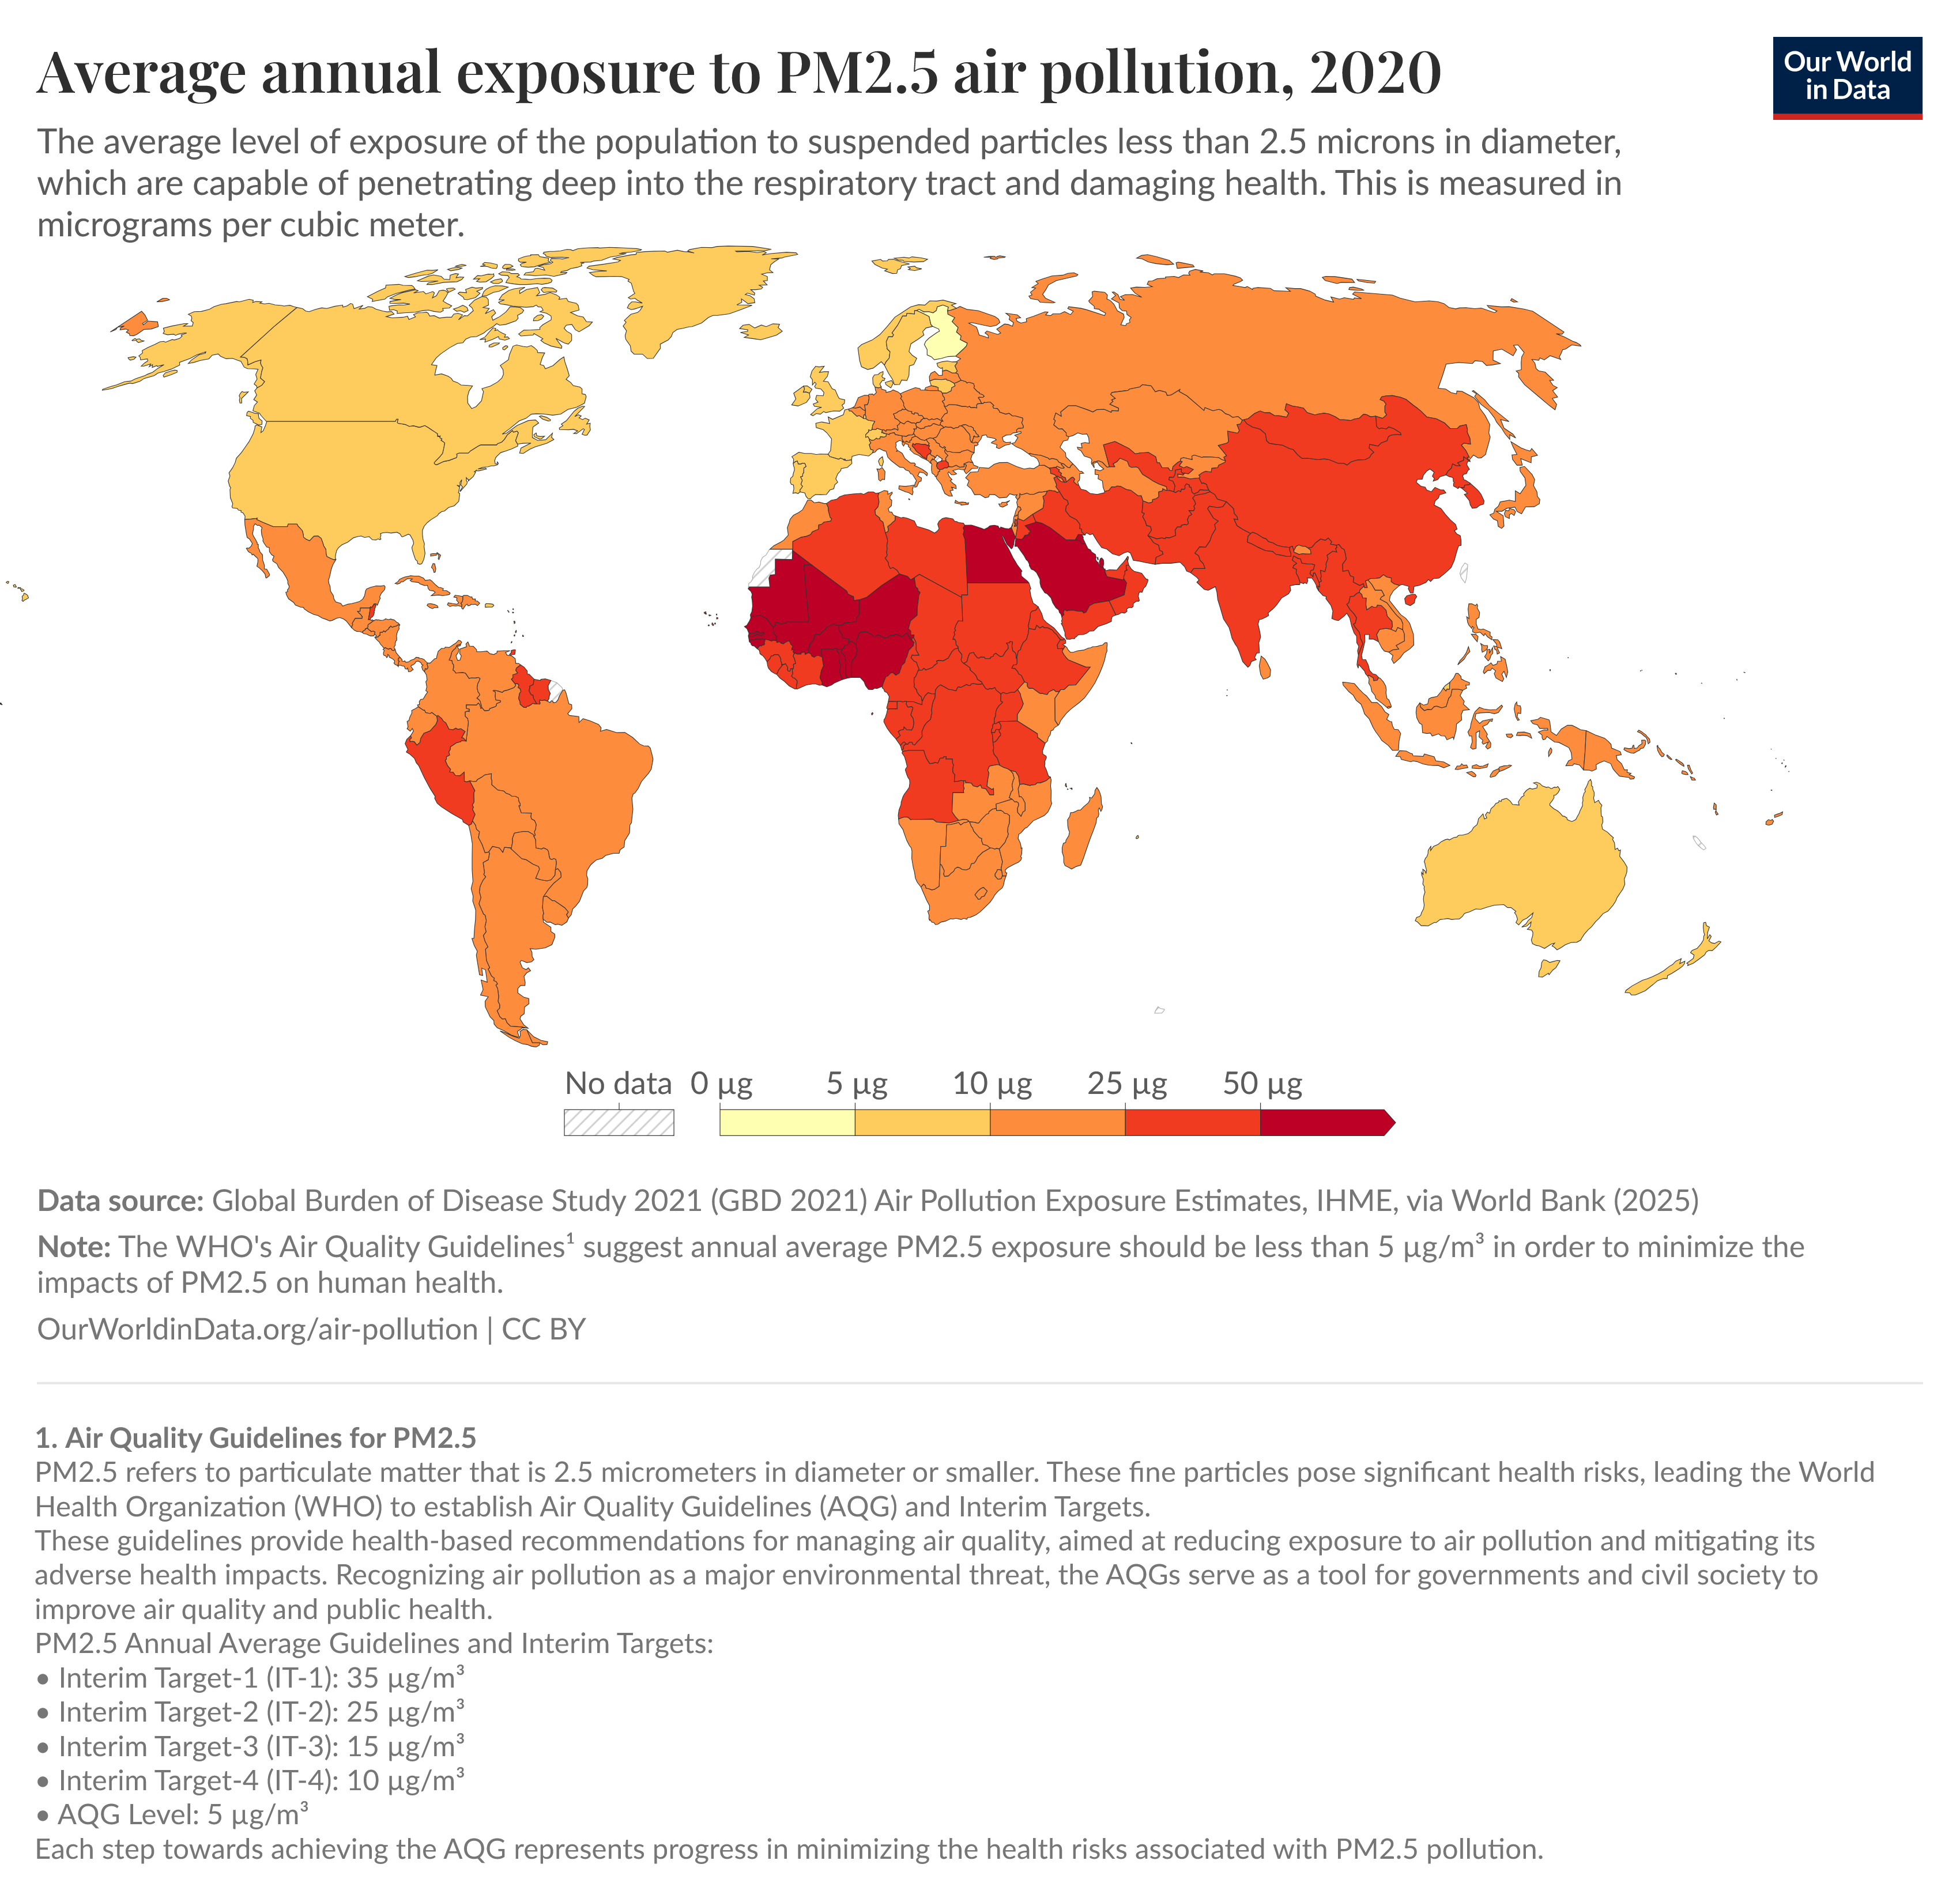
\includegraphics[width=\linewidth]{photos/average-exposure-pm25-pollution.png}
%   \caption{Royaume-Uni, XIX\textsuperscript{e} siècle}
% \end{column}

% % --- Right figure ---
% \begin{column}{0.48\textwidth}
%   \centering
%   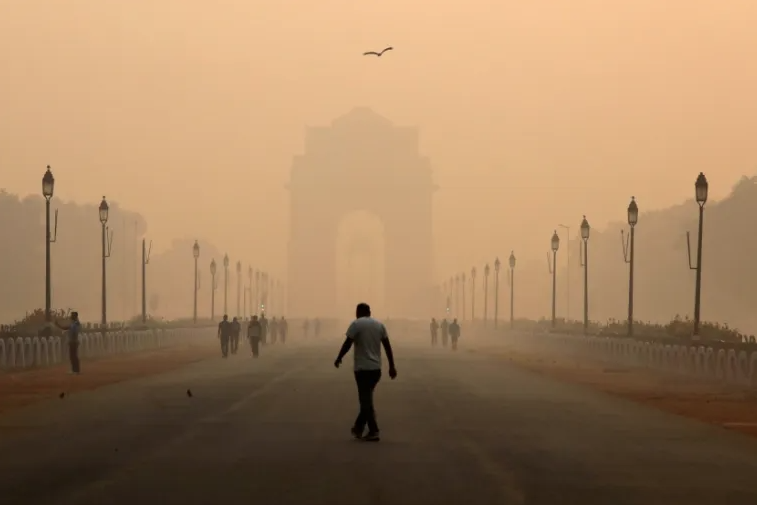
\includegraphics[width=\linewidth]{photos/india_gate_delhi_2018.png}
%   \caption{Inde, XXI\textsuperscript{e} siècle}
% \end{column}

% \end{columns}
% \end{figure}

% \end{frame}

\section{Namur Audition}

\begin{frame}

\vspace{1.0cm}

\centering
{\Large \textbf{Florian Münch}} \\[0.3cm]

{\small London School of Economics \\ (Chercheur postdoctoral, projet \textit{Productive and Inclusive Net Zero})} \\ 
\& \\
{\small King’s College London \\ (Responsable de module en économie environnementale)} \\[0.6cm]

{\small Audition pour le poste de Professeur assistant en économie} \\
{\small Université de Namur, 26 janvier 2026}

\vfill

\end{frame}

\begin{frame}{Structure de la Présentation}
\begin{enumerate}
    \item Présentation pédagogique : \textit{Régulation de la pollution sous incertitude (Weitzman, 1974)}  \\~\\
    \item Présentation de recherche : \textit{Stronger Together? Female Export Consortia}  \\~\\
    \item Programme de recherche
\end{enumerate}
\end{frame}


\begin{frame}{Présentation pédagogique: Agenda}

\textbf{Sujet :} La régulation de la pollution sous incertitude \\ (Martin Weitzman 1974 \textit{Prix vs Quantités})

\begin{enumerate}
    \item La pollution comme une externalité qui entraine une défaillance du marché et un excès de production \\~\\
    \item La problèmatique de Weitzman : réguler la pollution par les prix ou par les quantités ? \\~\\
    \item Résultat clé : le choix de l’instrument dépend de la relation entre coûts de réduction \& dommages liées a la pollution
\end{enumerate}

\end{frame}


\begin{frame}{Pourquoi s'intéresser a la pollution?}
\begin{itemize}
    \item Depuis la révolution industrielle: Croissance économique et hausse des revenus et du bien-être matériel sans précédent \\~\\
    
    \item Accompagnée également d’une pollution environnementale inédite \\~\\

    \item Conséquences massives pour les humains (santé) \& la nature (climat, biodiversité) \\~\\
    
    \item Vue économique de la pollution : \textbf{externalité}
        \begin{itemize}
            \item Définition: Les actions d'un agent affecte le bien-être des tiers sans en prendre compte dans ses décisions
            \item En conséquence, les decisions des acteurs du marché entraine un excès de pollution
        \end{itemize}
\end{itemize}
\end{frame}



%========================
% Slide: Externality
%========================

\begin{frame}{L'externalité et la surproduction (et la surpollution)}
\centering
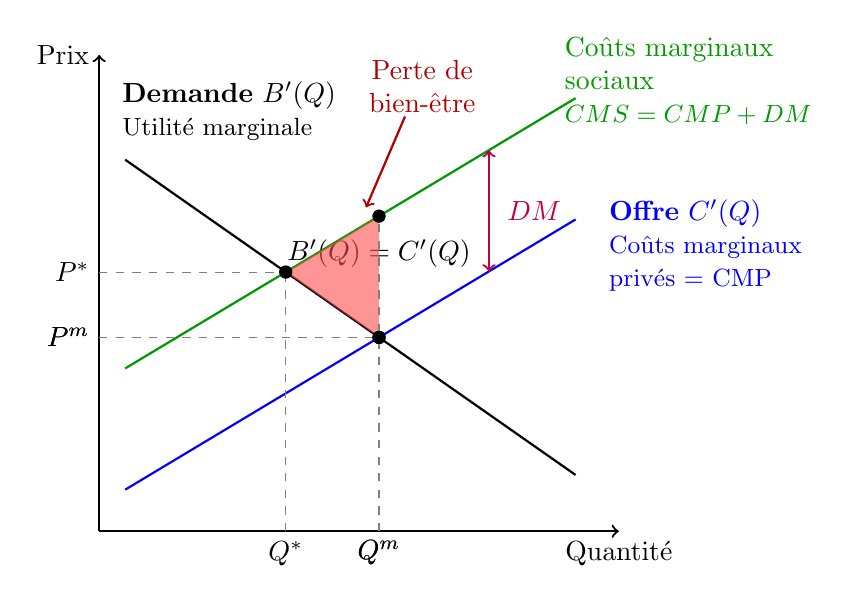
\begin{tikzpicture}[scale=1.1]

% Paramètres
\pgfmathsetmacro{\mD}{-0.7}    % pente demande (négative)
\pgfmathsetmacro{\bD}{4.5}     % intercept demande
\pgfmathsetmacro{\mS}{0.6}     % pente offre (CMP)
\pgfmathsetmacro{\bS}{0.3}     % intercept offre
\pgfmathsetmacro{\dm}{1.4}     % décalage vertical pour CMS

% Points d'équilibre
% Marché : Demande = Offre (CMP)
\pgfmathsetmacro{\Qm}{(\bD-\bS)/(\mS-\mD)}
\pgfmathsetmacro{\Pm}{\mS*\Qm+\bS}

% Optimal : Demande = CMS
\pgfmathsetmacro{\Qstar}{(\bD-\bS-\dm)/(\mS-\mD)}
\pgfmathsetmacro{\Pstar}{\mS*\Qstar+\bS+\dm}

% Point sur CMS à Qm (pour le triangle)
\pgfmathsetmacro{\CMSatQm}{\mS*\Qm+\bS+\dm}

% Axes
\draw[->, thick] (0,0) -- (6,0) node[below] {Quantité};
\draw[->, thick] (0,0) -- (0,5.5) node[left] {Prix};

% Courbe de demande B'(Q)
\draw[thick, black] (0.3, {\mD*0.3+\bD}) -- (5.5, {\mD*5.5+\bD});
\node[black, align=left] at (1.5, {\mD*0.5+\bD+0.7}) {\textbf{Demande} $B'(Q)$ \\ \small Utilité marginale};

% Courbe d'offre CMP = C'(Q)
\draw[thick, blue] (0.3, {\mS*0.3+\bS}) -- (5.5, {\mS*5.5+\bS});
\node[blue, align=left] at (7, {\mS*5.0+\bS}) {\textbf{Offre} $C'(Q)$ \\ \small Coûts marginaux \\ \small privés = CMP};

% Qm et Pm - équilibre de marché (slide 1 uniquement)
\onslide<1>{
\draw[dashed, gray] (\Qm, 0) -- (\Qm, \Pm);
\node[below] at (\Qm, 0) {$Q^m$};
\draw[dashed, gray] (0, \Pm) -- (\Qm, \Pm);
\node[left] at (0, \Pm) {$P^m$};
\filldraw[black] (\Qm, \Pm) circle (2pt);

% Label B'(Q) = C'(Q) au-dessus du point d'intersection (slide 1 uniquement)
\node[above] at (\Qm, \Pm + 0.7) {$B'(Q) = C'(Q)$};
}

% === Slide 2: Ajout CMS et tout le reste ===
\onslide<2->{

% Courbe CMS = CMP + DM (coûts marginaux sociaux)
\draw[thick, green!60!black] (0.3, {\mS*0.3+\bS+\dm}) -- (5.5, {\mS*5.5+\bS+\dm});
\node[green!60!black, align=left] at (6.8, {\mS*5.0+\bS+\dm+0.5}) {Coûts marginaux \\ sociaux \\ \small $CMS = CMP + DM$};

% Triangle de perte de bien-être (DWL)
\fill[red!70, opacity=0.6]
  (\Qstar, \Pstar) -- (\Qm, \Pm) -- (\Qm, \CMSatQm) -- cycle;


% Flèche et label DWL
\draw[->, thick, red!70!black] ({\Qm + 0.3}, {\CMSatQm + 1.15}) -- ({\Qm - 0.15}, {\CMSatQm + 0.1});
\node[red!70!black, align=center] at ({\Qm + 0.5}, {\CMSatQm + 1.5}) {Perte de \\ bien-être};

% Q* et P*
\draw[dashed, gray] (\Qstar, 0) -- (\Qstar, \Pstar);
\node[below] at (\Qstar, 0) {$Q^*$};
\draw[dashed, gray] (0, \Pstar) -- (\Qstar, \Pstar);
\node[left] at (0, \Pstar) {$P^*$};

% Qm - ligne verticale jusqu'à CMS
\draw[dashed, gray] (\Qm, 0) -- (\Qm, \CMSatQm);
\node[below] at (\Qm, 0) {$Q^m$};
\draw[dashed, gray] (0, \Pm) -- (\Qm, \Pm);
\node[left] at (0, \Pm) {$P^m$};

% Flèche double entre CMP et CMS pour montrer DM
\pgfmathsetmacro{\xDM}{4.5}
\pgfmathsetmacro{\yCMP}{\mS*\xDM+\bS}
\pgfmathsetmacro{\yCMS}{\mS*\xDM+\bS+\dm}
\draw[<->, thick, purple] (\xDM, \yCMP) -- (\xDM, \yCMS);
\node[purple, right] at (\xDM + 0.1, {(\yCMP+\yCMS)/2}) {$DM$};

% Points d'intersection
\filldraw[black] (\Qstar, \Pstar) circle (2pt);
\filldraw[black] (\Qm, \Pm) circle (2pt);
\filldraw[black] (\Qm, \CMSatQm) circle (2pt);

}

\end{tikzpicture}
\end{frame}

% A dire
% Niveau de production du marche plus elevee que le niveau de production optimal
% Ceci est liee au fait que les producteurs ne prennent en compte que leur couts marginaux de production, et n'est pas les couts externent, p.ex. tous les couts medicaux causes par la prooduction, dans leur choice du q optimal. 

% Nous, autant qu'economistes, considerent ceci une defaillance de marche, car les droits de propriete ne sont pas complets; autrements dit, les producteurs n'internalisent qu'une partie des couts qu'ils causent

% La defaillance de marche justifie l'intervention de l'etat pour reduire le niveau de production (et de pollution liee a la production) au niveau optimal


%========================
% Slide: Weitzman 1 + MAC-MD definition
%========================

% \begin{frame}{Externalité environnementale et défaillance du marche: Comment atteindre le niveau optimal de pollution ?}

% \begin{itemize}
%     \item<1-> \textbf{Définition économique du niveau optimal de la pollution:}
%     \begin{itemize}
%         \item<1-> $C'(Q) = B'(Q) $
%         \item<1-> \textit{Attention}: Q = pollution
%         \item<1-> $C'(Q)$: coûts marginaux d’abattement (CMA) 
%         \item<1-> $B'(Q) $: dommage marginal (bénéfices marginaux d’abattement (BMA))
%     \end{itemize}
% \end{itemize}

% \end{frame}

% A dire:
% ds l'equilibre, les couts de reduction de la pollution sont egale au dommage cause

% \begin{frame}{Le problème: Comment atteindre l'optimum social de pollution?}

% \only<1>{
% \begin{itemize}
%     \item<1-> \textbf{Weitzman (1974) : deux options pour controler la pollution}
%     \begin{enumerate}
%         \item<1-> Réguler le prix
%         \item<1-> Réguler la quantité
%     \end{enumerate}        
% \end{itemize}
% }
% \end{frame}

\begin{frame}{Comment atteindre l'optimum social de pollution? \\ }
\centering
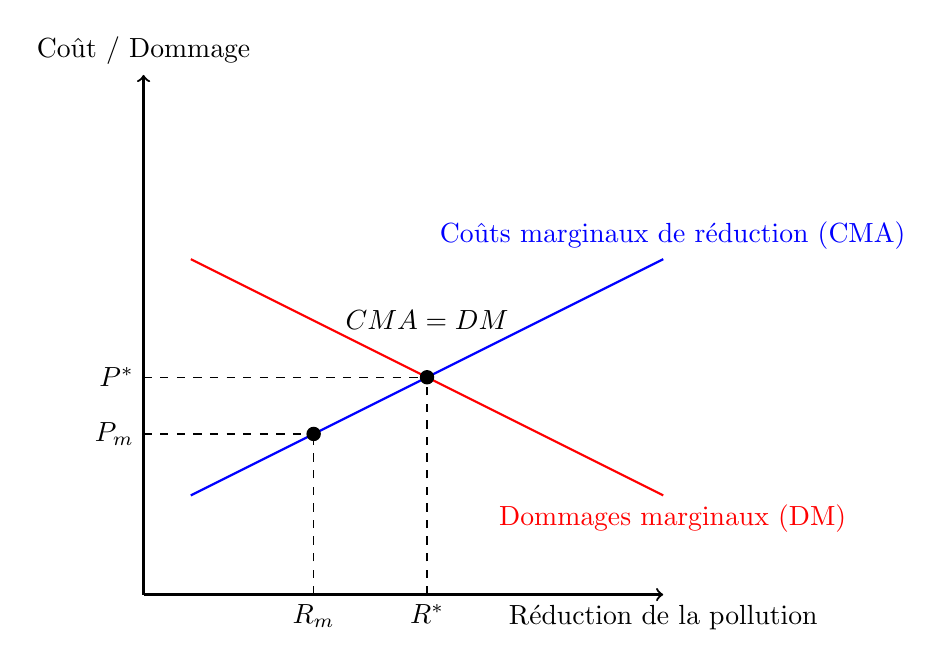
\begin{tikzpicture}[scale=1.2]

% Paramètres
\pgfmathsetmacro{\m}{0.5}   % pente
\pgfmathsetmacro{\bA}{0.8}  % intercept CMA
\pgfmathsetmacro{\k}{3.8}   % intercept DM

% Intersection CMA = DM (optimum social)
\pgfmathsetmacro{\Rstar}{(\k-\bA)/(2*\m)}
\pgfmathsetmacro{\Pstar}{\m*\Rstar+\bA}

% Niveau de marché (Rm < R*)
\pgfmathsetmacro{\Rm}{\Rstar-1.2}
\pgfmathsetmacro{\Pm}{\m*\Rm+\bA}

% Axes (toujours visibles)
\draw[->, thick] (0,0) -- (5.5,0) node[below] {Réduction de la pollution};
\draw[->, thick] (0,0) -- (0,5.5) node[above] {Coût / Dommage};



% -----------------------------------
% 1) CMA seule
% -----------------------------------
\onslide<2->{
\draw[thick, blue] (0.5, {\m*0.5+\bA}) -- (5.5, {\m*5.5+\bA});
\node[blue] at (5.6, {\m*5.5+\bA+0.25}) {Coûts marginaux de réduction (CMA)};
}
% -----------------------------------
% 2) DM seul
% -----------------------------------
\onslide<3->{
\draw[thick, red] (0.5, {\k-\m*0.5}) -- (5.5, {\k-\m*5.5});
\node[red] at (5.6, {\k-\m*5.5-0.25}) {Dommages marginaux (DM)};
}

% -----------------------------------
% 3) Optimum social (R*, P*, CMA = DM)
% -----------------------------------
\onslide<4->{
% Point optimal
\filldraw[black] (\Rstar,\Pstar) circle (2pt);
% R*
\draw[dashed] (\Rstar,0) -- (\Rstar,\Pstar);
\node[below] at (\Rstar,0) {$R^*$};
% P*
\draw[dashed] (0,\Pstar) -- (\Rstar,\Pstar);
\node[left] at (0,\Pstar) {$P^*$};
}

% Label CMA = DM au-dessus du point d'intersection (version 4 uniquement)
\onslide<4>{
\node[above] at (\Rstar, \Pstar + 0.4) {$CMA = DM$};
}

% -----------------------------------
% 4) Niveau de marché (Rm, Pm)
% -----------------------------------
\onslide<5->{
% Point de marché
\filldraw[black] (\Rm,\Pm) circle (2pt);
% Rm
\draw[dashed] (\Rm,0) -- (\Rm,\Pm);
\node[below] at (\Rm,0) {$R_m$};
% Pm
\draw[dashed] (0,\Pm) -- (\Rm,\Pm);
\node[left] at (0,\Pm) {$P_m$};
}

\end{tikzpicture}

\end{frame}



\begin{frame}{Prix ou quantité ? La problématique de Weitzman (1974)}
\centering
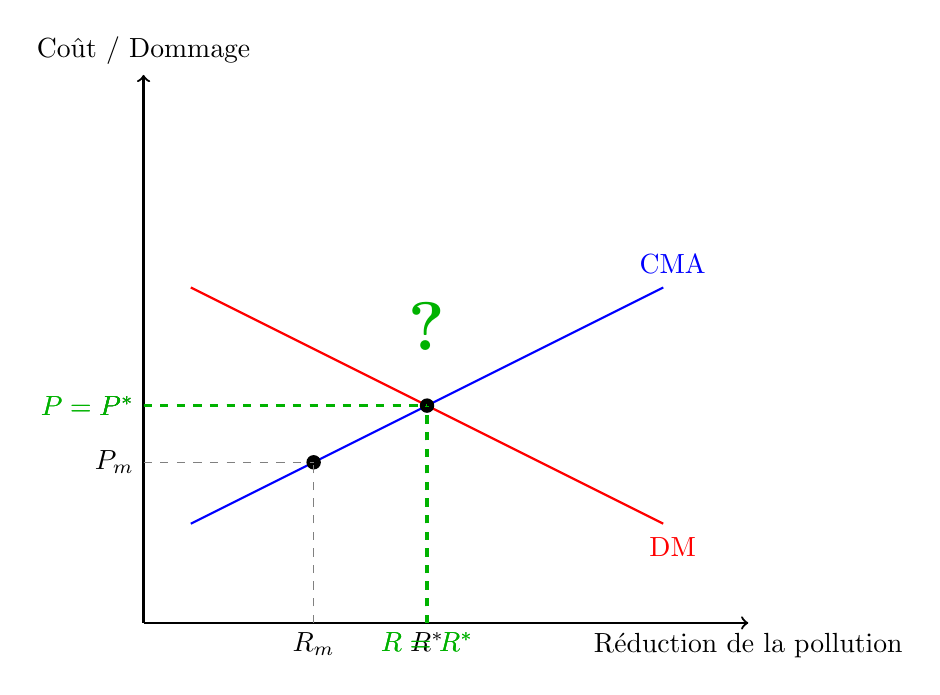
\begin{tikzpicture}[scale=1.2]
% Paramètres
\pgfmathsetmacro{\m}{0.5}
\pgfmathsetmacro{\bA}{0.8}
\pgfmathsetmacro{\k}{3.8}
% Intersection CMA = DM (optimum social)
\pgfmathsetmacro{\Rstar}{(\k-\bA)/(2*\m)}
\pgfmathsetmacro{\Pstar}{\m*\Rstar+\bA}
% Niveau de marché (Rm < R*)
\pgfmathsetmacro{\Rm}{\Rstar-1.2}
\pgfmathsetmacro{\Pm}{\m*\Rm+\bA}
% Axes
\draw[->, thick] (0,0) -- (6.4,0) node[below] {Réduction de la pollution};
\draw[->, thick] (0,0) -- (0,5.8) node[above] {Coût / Dommage};
% CMA
\draw[thick, blue] (0.5, {\m*0.5+\bA}) -- (5.5, {\m*5.5+\bA});
\node[blue] at (5.6, {\m*5.5+\bA+0.25}) {CMA};
% DM
\draw[thick, red] (0.5, {\k-\m*0.5}) -- (5.5, {\k-\m*5.5});
\node[red] at (5.6, {\k-\m*5.5-0.25}) {DM};
% Point optimal
\filldraw[black] (\Rstar,\Pstar) circle (2pt);
% Lignes pointillées standard (gris)
\draw[dashed, gray] (\Rstar,0) -- (\Rstar,\Pstar);
\draw[dashed, gray] (0,\Pstar) -- (\Rstar,\Pstar);
% Point de marché
\filldraw[black] (\Rm,\Pm) circle (2pt);
\draw[dashed, gray] (\Rm,0) -- (\Rm,\Pm);
\draw[dashed, gray] (0,\Pm) -- (\Rm,\Pm);
\node[below] at (\Rm,0) {$R_m$};
\node[left] at (0,\Pm) {$P_m$};

% -----------------------------------
% 1) Quantité (ligne verticale en vert)
% -----------------------------------
\onslide<1>{
\draw[dashed, very thick, green!70!black] (\Rstar,0) -- (\Rstar,\Pstar);
\node[below, green!70!black] at (\Rstar,0) {$R = R^*$};
\node[left] at (0,\Pstar) {$P^*$};
}

% -----------------------------------
% 2) Prix (ligne horizontale en vert)
% -----------------------------------
\onslide<2>{
\draw[dashed, very thick, green!70!black] (0,\Pstar) -- (\Rstar,\Pstar);
\node[below] at (\Rstar,0) {$R^*$};
\node[left, green!70!black] at (0,\Pstar) {$P = P^*$};
}

% -----------------------------------
% 3) Prix + Quantité + ?
% -----------------------------------
\onslide<3>{
\draw[dashed, very thick, green!70!black] (\Rstar,0) -- (\Rstar,\Pstar);
\draw[dashed, very thick, green!70!black] (0,\Pstar) -- (\Rstar,\Pstar);
\node[below, green!70!black] at (\Rstar,0) {$R = R^*$};
\node[left, green!70!black] at (0,\Pstar) {$P = P^*$};
\node[green!70!black, font=\Huge\bfseries] 
at (\Rstar,\Pstar) [yshift=1cm] {?};
}

\end{tikzpicture}
\end{frame}


% \begin{frame}{Externalité environnementale et défaillance du marche: Comment atteindre l’optimum de pollution ?}

% \begin{itemize}
%     \item<1-> \textbf{Définition économique du niveau optimal de pollution :}
%     \begin{itemize}
%         \item<1-> $C'(Q) = B'(Q) $
%         \item<1-> \textit{Attention}: Q = pollution
%         \item<1-> $C'(Q)$: coûts marginaux d’abattement (CMA) 
%         \item<1-> $B'(Q) $: dommage marginal (bénéfices marginaux d’abattement (BMA))
%     \end{itemize}

%     \vspace{0.4cm}
    
%     \item<1-> \textbf{Weitzman (1974) : deux options}
%     \begin{enumerate}
%         \item<1-> Réguler le prix
%         \item<1-> Réguler la quantité
%     \end{enumerate}
% \end{itemize}

% \end{frame}


%========================
% Slide: MAC-MD plus quantity and price regulation
%========================
% \begin{frame}{Reduction (Abattement) des Pollutions: Par Quantite ou Prix?}

% \centering
% \only<1>{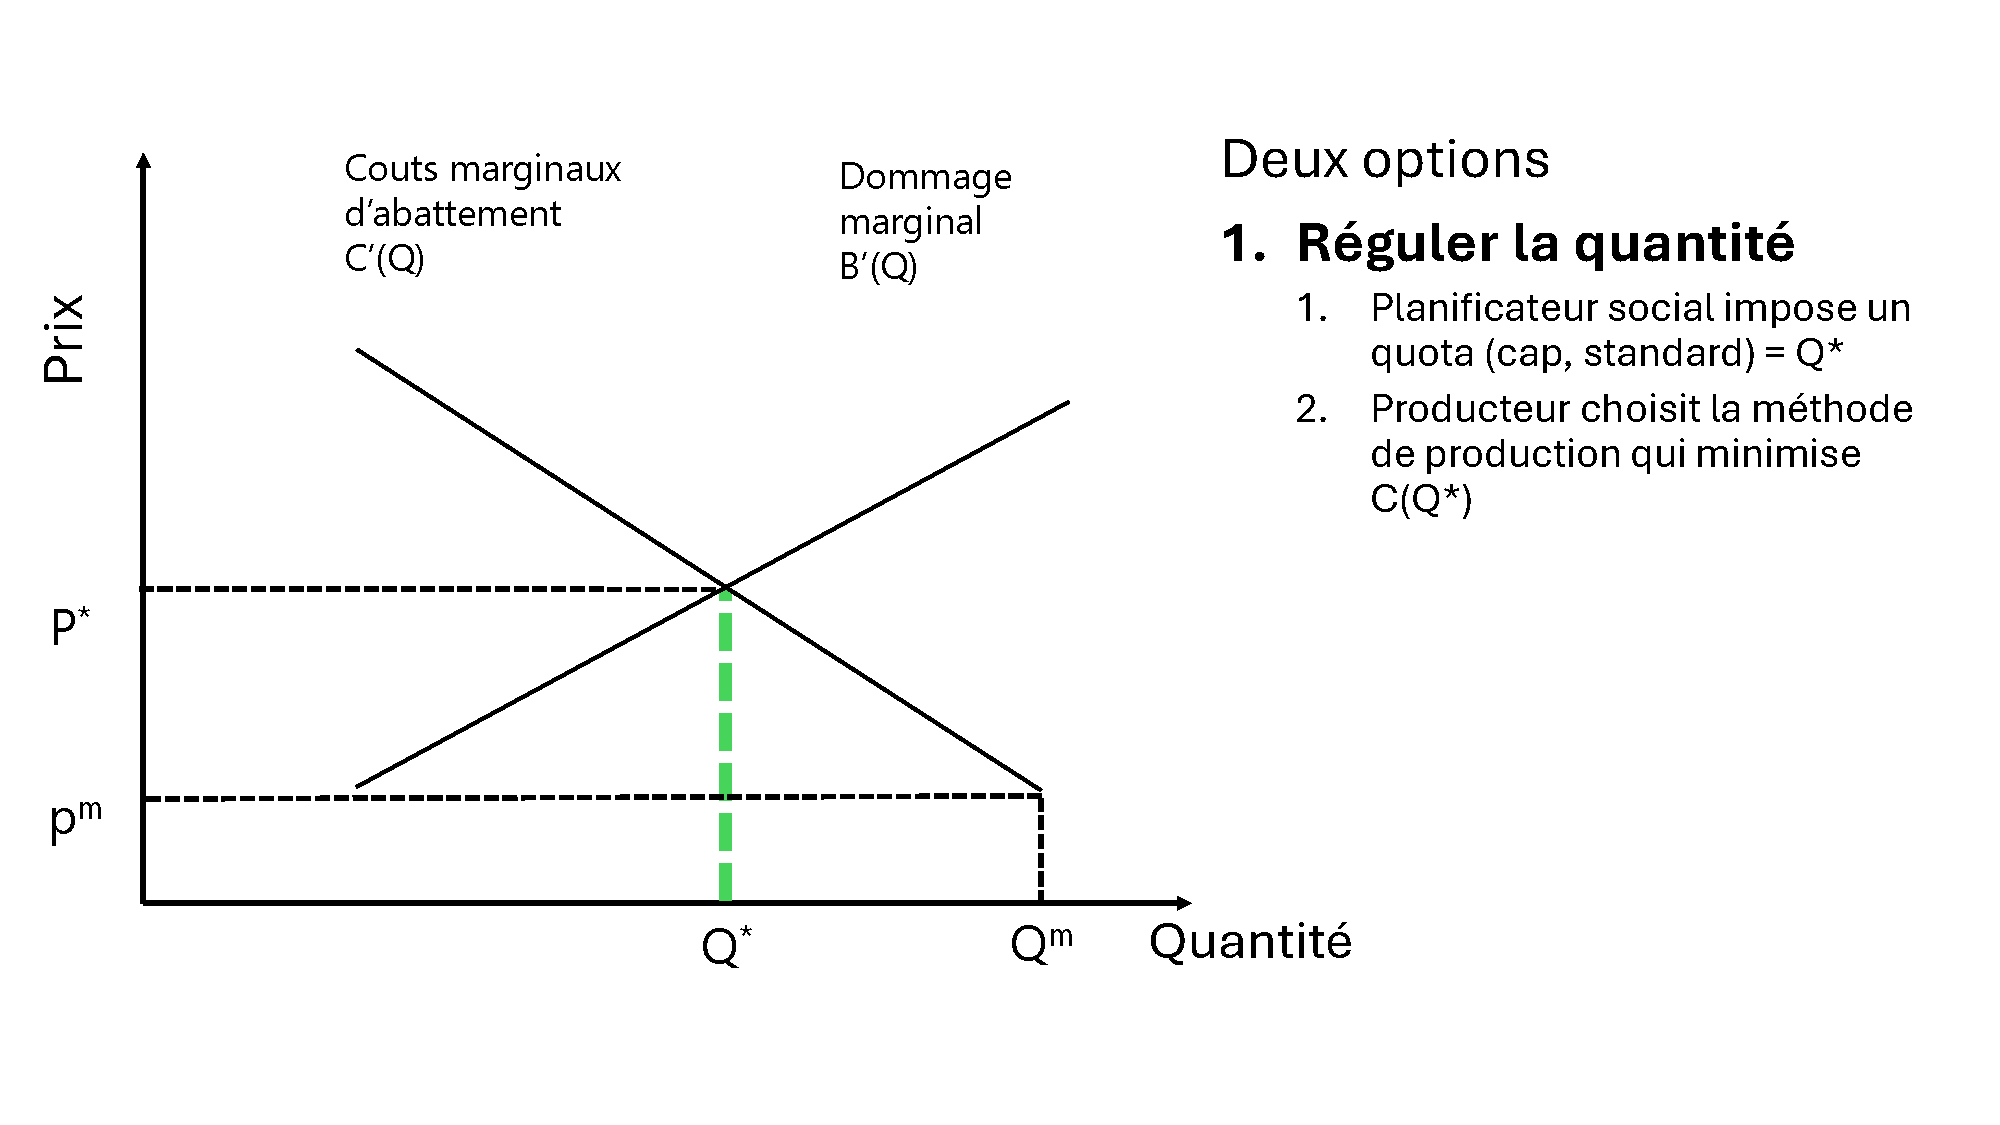
\includegraphics[width=1.05\textwidth]{mac_md_curves/mac_md_quantite.pdf}}
% \only<2>{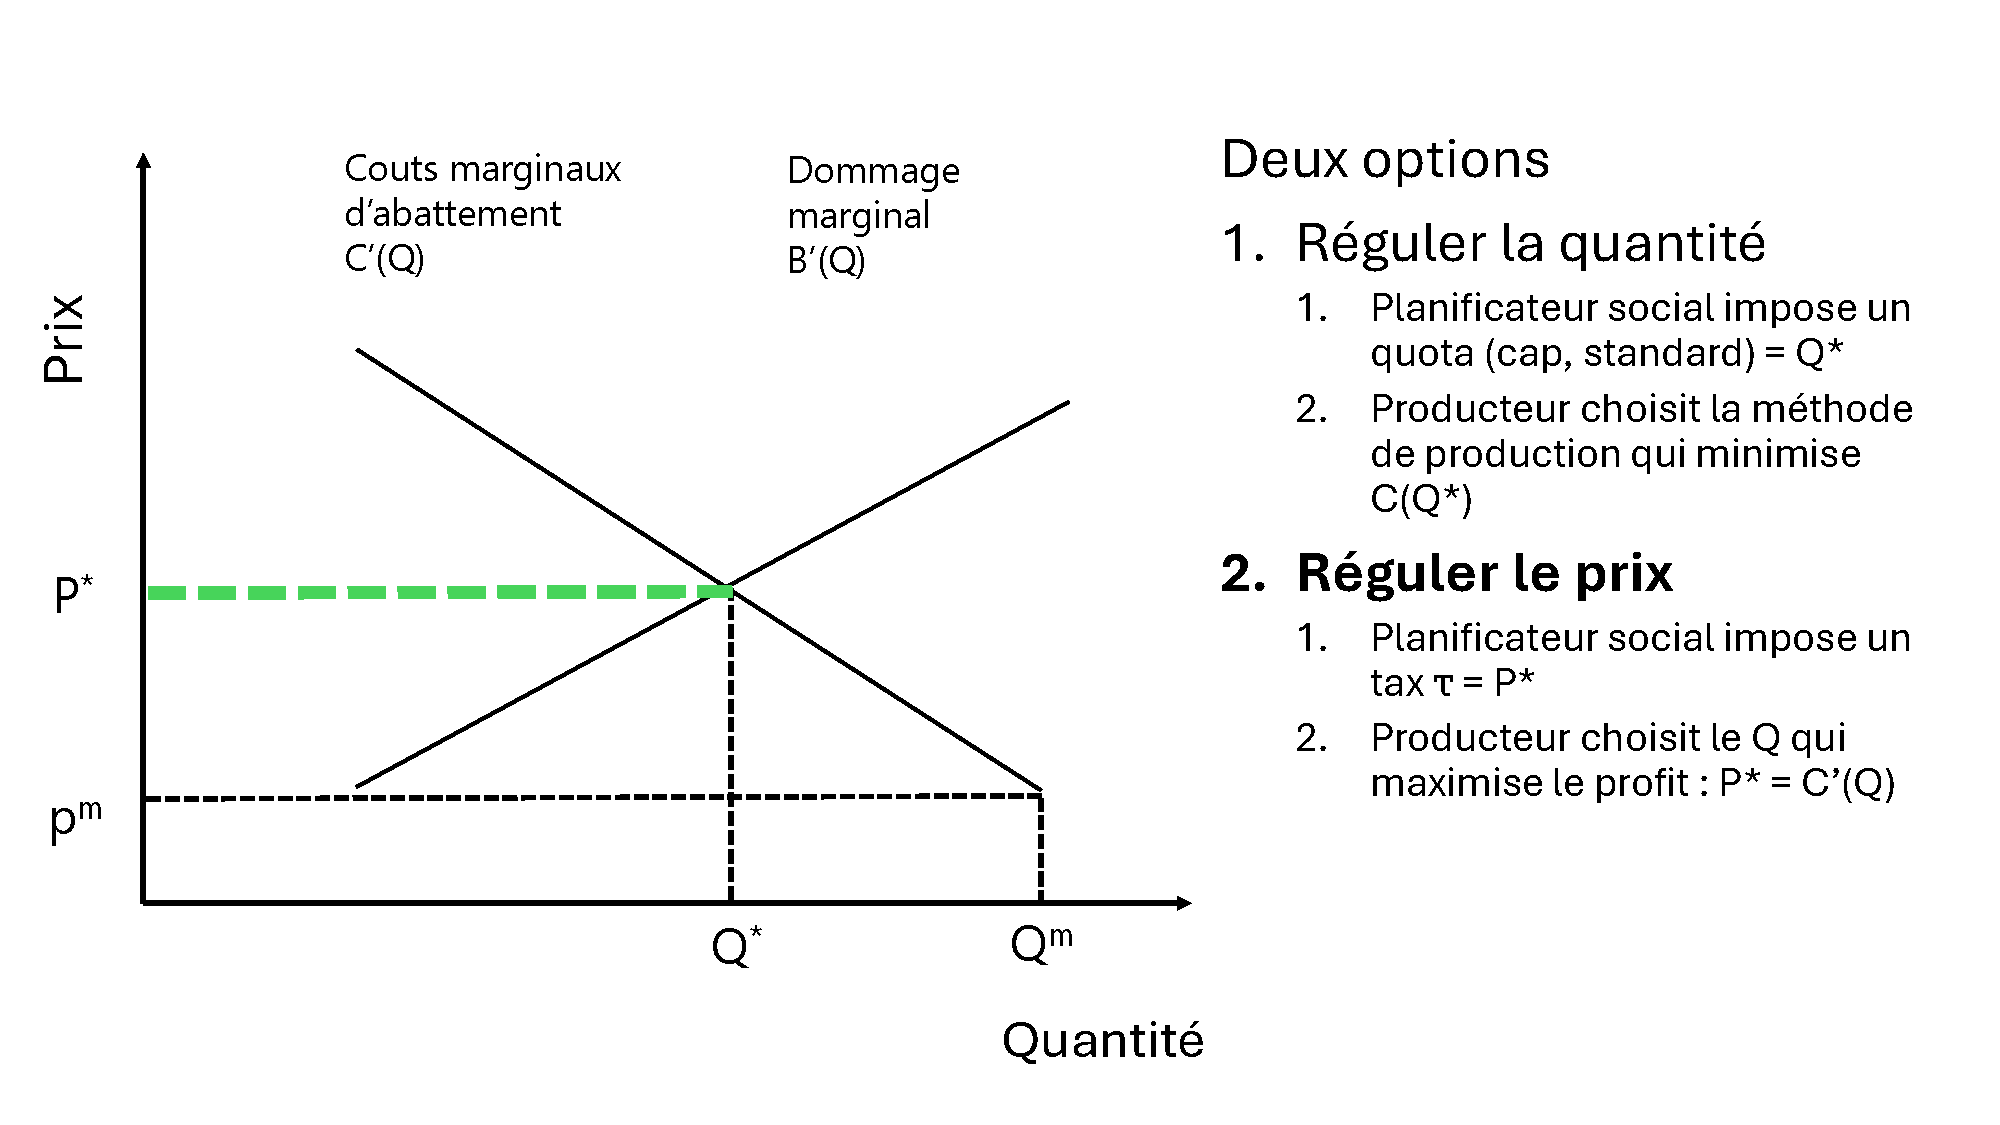
\includegraphics[width=1.05\textwidth]{mac_md_curves/mac_md_prix.pdf}}
% \only<3>{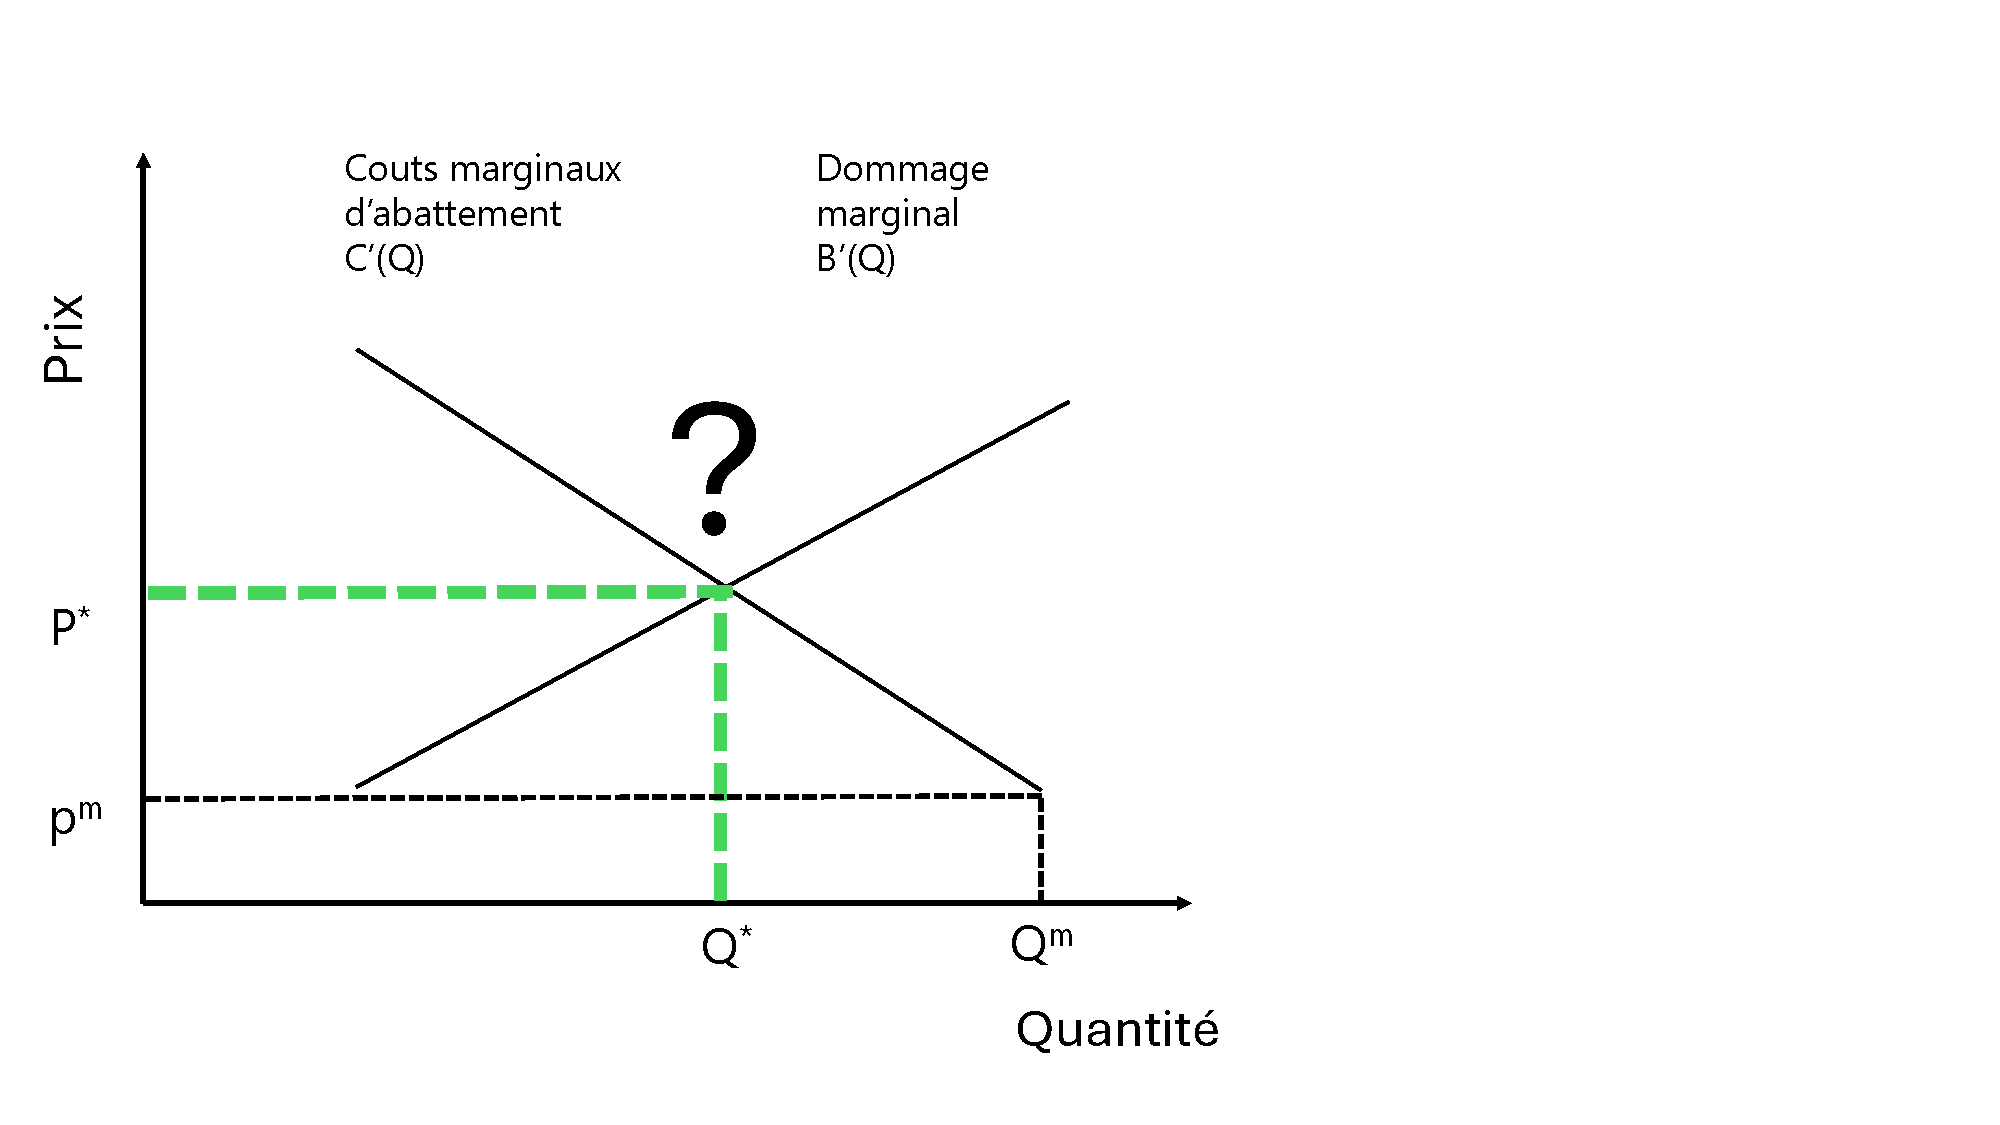
\includegraphics[width=1.05\textwidth]{mac_md_curves/mac_md_question.pdf}
%     \item \textbf{Question de savoir :} la régulation par les prix ou par les quantités est-elle plus efficace pour contrôler la pollution ?
% }
% \end{frame}


% \begin{frame}{Externalité environnementale et défaillance du marche: Comment atteindre l’optimum social ?}

% \begin{itemize}
%     \item \textbf{Définition économique de l’optimum social :}
%     \begin{itemize}
%         \item $B'(Q) = C'(Q)$
%         \item Équilibrer les coûts marginaux d’abattement (CMA) et les bénéfices marginaux d’abattement (BMA)
%     \end{itemize}

%     \vspace{0.4cm}
    
%     \item \textbf{Weitzman (1974) : deux options}
%     \begin{enumerate}
%         \item Réguler le prix
%         \item Réguler la quantité
%     \end{enumerate}

%     \vspace{0.4cm}

%     \item \textbf{Question de savoir :} la régulation par les prix ou par les quantités est-elle plus efficace pour contrôler la pollution ?
% \end{itemize}

% \end{frame}


% \begin{frame}{Weitzman (1974) : rôle de $B''$ et $C''$}

% \centering
% \begin{tikzpicture}[scale=1.1]

% % Axes
% \draw[->] (0,0) -- (6,0) node[right] {Abattement $q$};
% \draw[->] (0,0) -- (0,4.5) node[above] {Coût / Bénéfice marginal};

% % MAC curve (upward sloping, convex)
% \draw[thick, blue, domain=0.2:5.5, smooth] plot (\x, {0.3 + 0.1*\x + 0.08*\x*\x});
% \node[blue] at (5.2,4.1) {MAC $= C'(q)$};
% \node[blue] at (4.2,3.2) {$C''>0$};

% % MB curve (downward sloping, concave)
% \draw[thick, red, domain=0.2:5.5, smooth] plot (\x, {4.2 - 0.5*\x - 0.05*\x*\x});
% \node[red] at (5.1,0.7) {MB $= B'(q)$};
% \node[red] at (3.2,2.0) {$B''<0$};

% % Intersection point
% \draw[dashed] (2.6,0) -- (2.6,2.2);
% \draw[dashed] (0,2.2) -- (2.6,2.2);
% \filldraw (2.6,2.2) circle (2pt);

% \node at (2.6,-0.3) {$q^*$};
% \node at (-0.4,2.2) {$MAC=MB$};

% \end{tikzpicture}

% \vspace{0.3cm}

% \textbf{Weitzman :} sous incertitude, le choix entre prix et quantités dépend de la courbure relative des fonctions de coûts et de bénéfices, c’est-à-dire de $C''$ et $B''$.

% \end{frame}




%========================
% Slide B: Uncertainty
%========================

\begin{frame}{Incertitude sur les coûts de reduction \& les dommages de la pollution}

\begin{itemize}
  \item<1-> En cas d'information parfaite, $q^*$ et $p^*$ sont connus et la régulation par prix ou quantité est équivalente.
  
  \item<2-> En réalité, le planificateur social manque d'information \& les C\&B d'abattement de la pollution sont incertains :
  \[
  CMA(q,\textcolor{blue}{\theta}) \quad ; \quad DM(q,\textcolor{red}{\eta}),
  \]
  où \textcolor{blue}{$\theta$} et \textcolor{red}{$\eta$} représentent des paramètres d'incertitude.
\end{itemize}

\vspace{0.2cm}

\onslide<3->{
\textbf{Implication :}
\begin{itemize}
  \item<3-> Le planificateur social prend donc des décisions approximatifs, nécessairement imparfaites (sous-optimales).
  \item<4-> Ex.: $p_r<p*$: excès de pollution; $q_r < q*$: excès des coûts.
  \item<5-> Arbitrage: fixer $p_r$: "certitude des coûts" et fixer $q_r$ "certitude des dommages".

\end{itemize}
}

\end{frame}



%========================
% Slide D+E: Comparison and approximation
%========================
\begin{frame}{Comparer les instruments prix et quantité}
%----------------------------------
% Step 1: simple criterion + Wprix
%----------------------------------
\onslide<1->{
\textbf{Critère de comparaison $\Delta$ ("perte relative de bien-être")}
\vspace{0.05cm}
\[
\Delta = W^{\text{prix}} - W^{\text{quantité}}
\]
}
\onslide<2->{
\vspace{-0.2cm} % réduit l'espace entre les deux formules
\[
\text{où } W^{prix} = \mathbb{E}\Big[B\big(q(p,\textcolor{red}{\eta})\big) - C\big(q(p,\textcolor{blue}{\theta}),\textcolor{blue}{\theta}\big)\Big].
\]
}
%----------------------------------
% Step 2: definition of W^{prix}
%----------------------------------
\only<3>{  % Changed from \onslide to \only
\vspace{-0.6cm} % réduit l'espace avant itemize
\begin{itemize}
  \item $\Delta > 0$ : la régulation par les prix est préférable.
  \item $\mathbb{E}$ : L'espérance du bien-être moyen sur l'ensemble des réalisations r possibles des C\&B.
\end{itemize}
\vspace{0.2cm}
}
%----------------------------------
% Step 3: Taylor approximation
%----------------------------------
\onslide<4->{
\textbf{Approximation locale de $\Delta$ ("perte relative de bien-être")}
\vspace{0.05cm}
\[
\Delta \approx \frac{\sigma^2}{2(C'')^2}\big(B'' + C''\big).
\]
\begin{itemize}
  \item $C''$ : pente des coûts marginaux d'abattement (CMA),
  \item $B''$ : pente des dommages marginaux (DM).
\end{itemize}
\vspace{0.05cm}
\textbf{Résultat:}  
$B'' + C''$ détermine l'instrument optimal.
}
\end{frame}

%========================
% Slide: Visualization of steep vs flat MAC & MD curves
%========================
% \begin{frame}{B'' et C'' visualisée: }


% \centering
% \only<1>{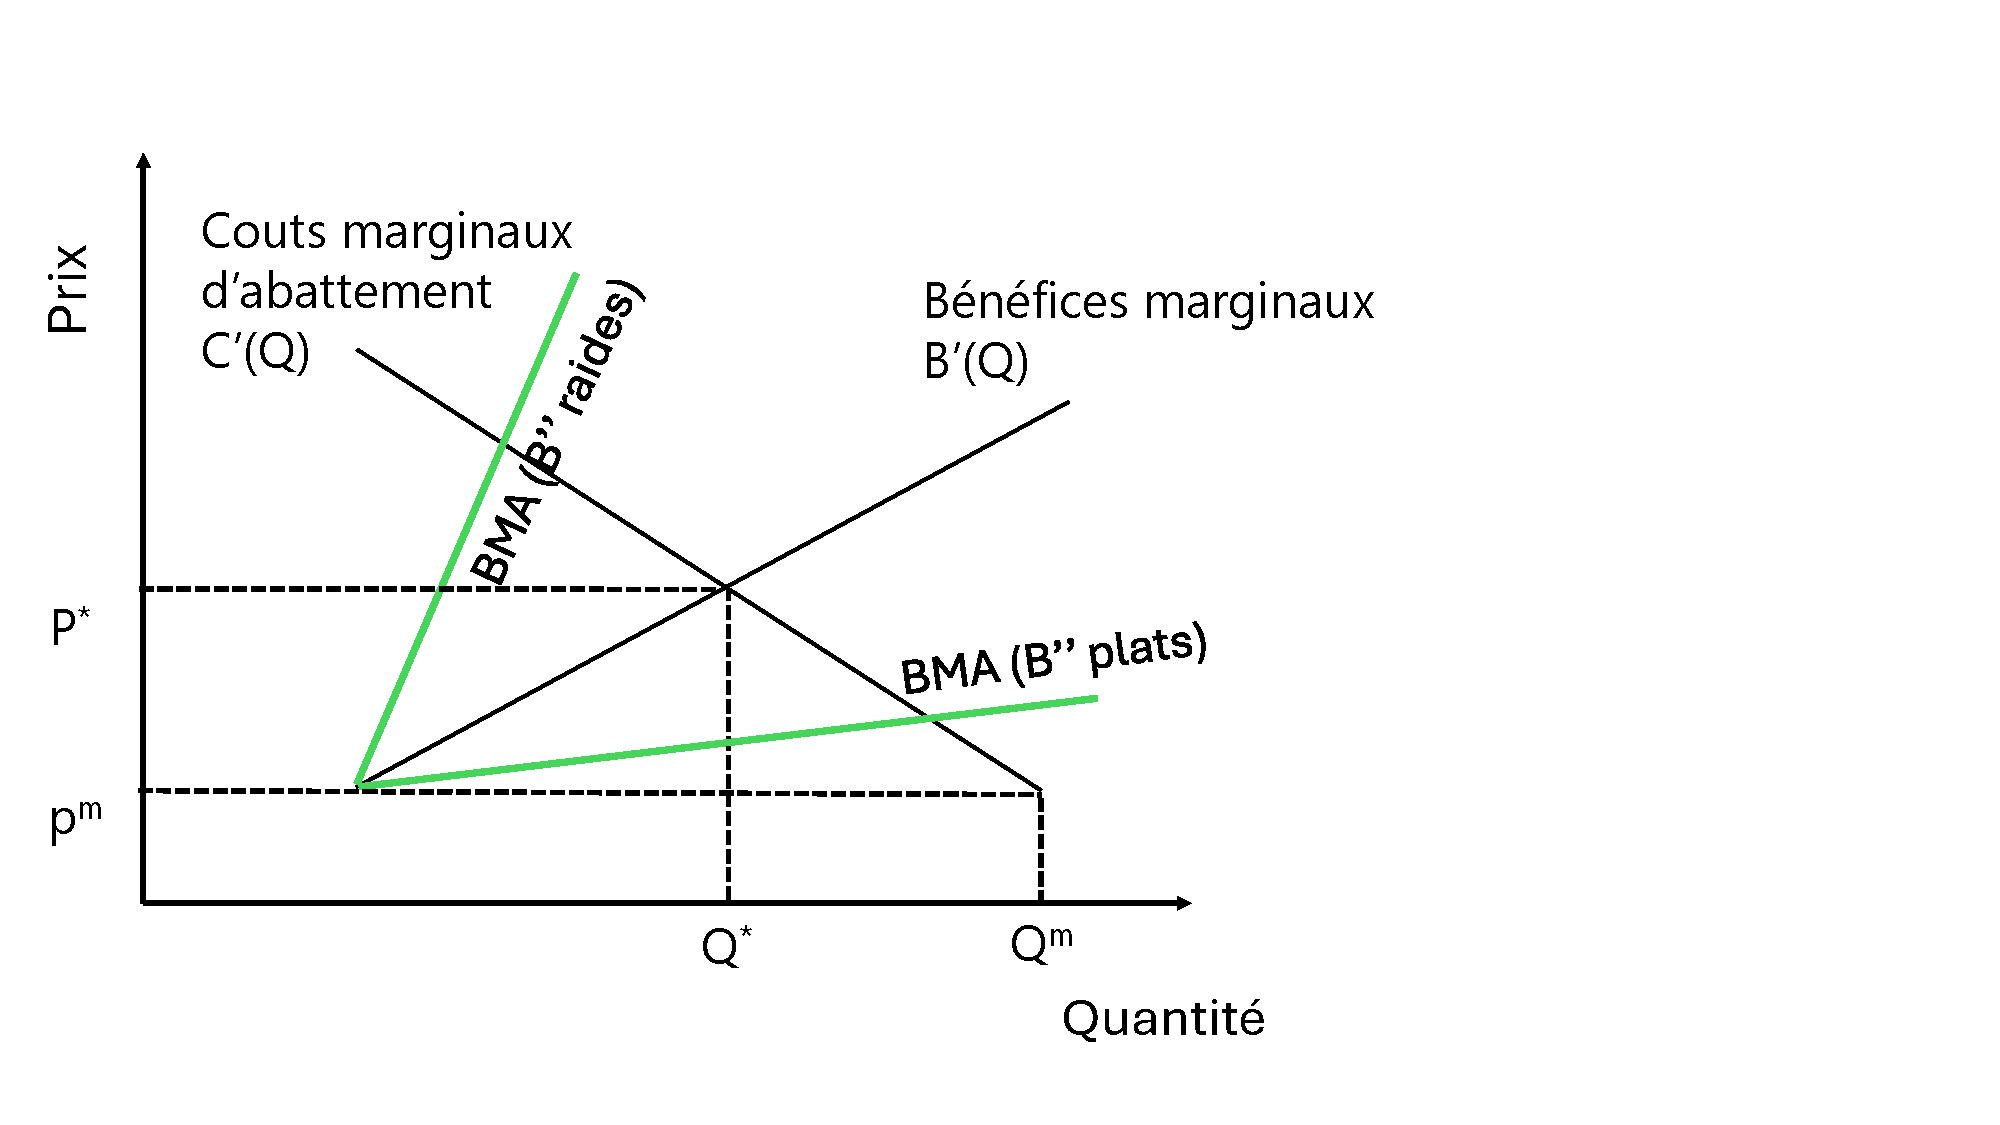
\includegraphics[width=1.1\textwidth]{mac_md_curves/md_bma_raides.pdf}}
% \only<2>{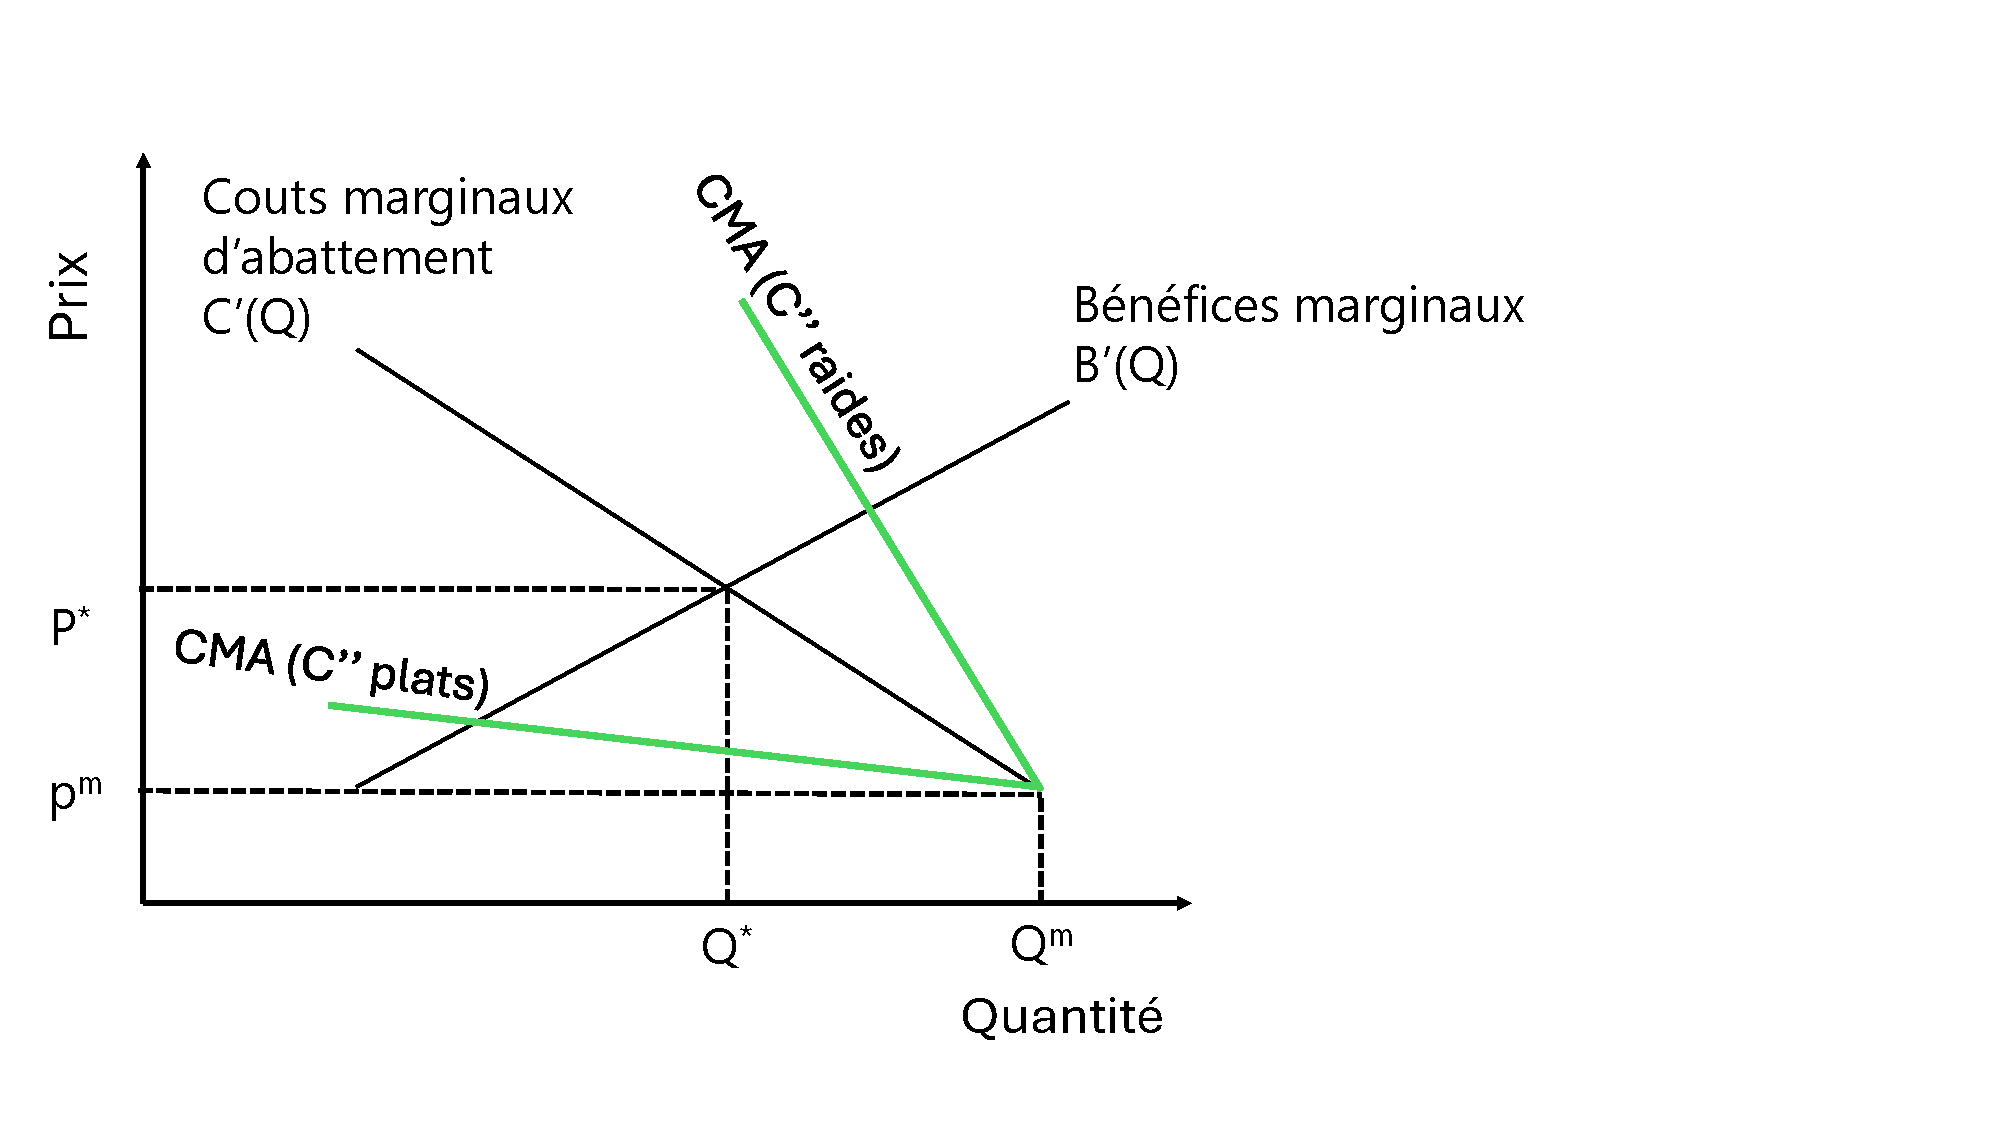
\includegraphics[width=1.1\textwidth]{mac_md_curves/md_bma_plats.pdf}
% }

% \end{frame}


\begin{frame}{Taxe vs quota : curbe DM plate}

\centering
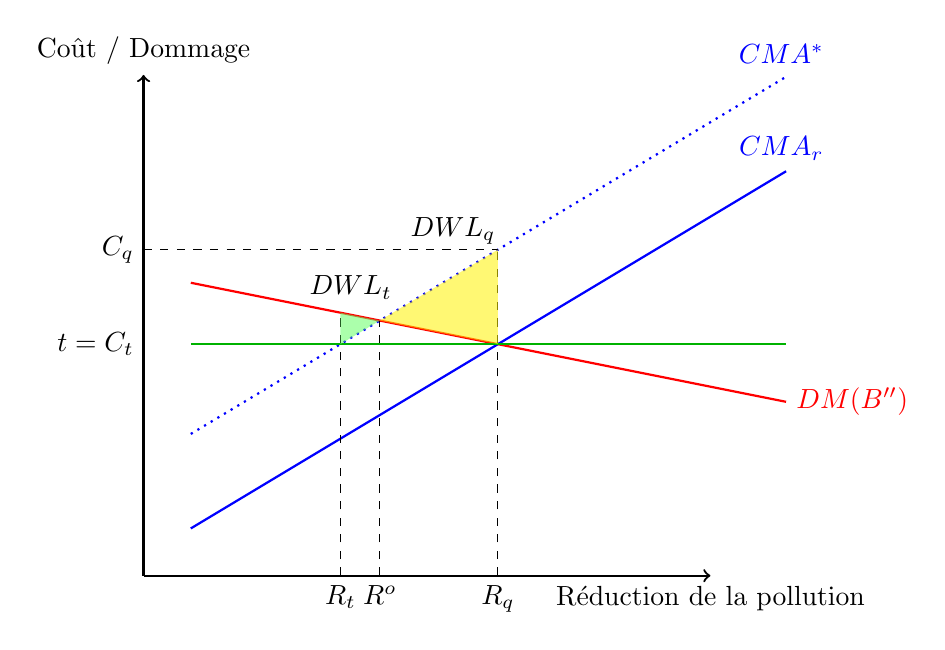
\begin{tikzpicture}[scale=1.2]

% Paramètres (MD relativement plat)
\pgfmathsetmacro{\m}{0.6}
\pgfmathsetmacro{\bE}{0.2}
\pgfmathsetmacro{\bA}{1.2}
\pgfmathsetmacro{\k}{3.2}
\pgfmathsetmacro{\d}{0.2} % MD plat

% Point de pivot : intersection CMAr et DM
\pgfmathsetmacro{\Rpivot}{(\k-\bE)/(\m+\d)}
\pgfmathsetmacro{\tlevel}{\m*\Rpivot+\bE}  % taxe passe par CMAr au pivot

% Points clés
\pgfmathsetmacro{\Ro}{(\k-\bA)/(\m+\d)}
\pgfmathsetmacro{\yRo}{\m*\Ro+\bA}

\pgfmathsetmacro{\Rq}{(\k-\bE)/(\m+\d)}
\pgfmathsetmacro{\yRq}{\m*\Rq+\bE}

% Rt : intersection CMA* et taxe
\pgfmathsetmacro{\Rt}{(\tlevel-\bA)/\m}
\pgfmathsetmacro{\yMDatRt}{\k-\d*\Rt}

\pgfmathsetmacro{\Cq}{\m*\Rq+\bA}

% Axes
\draw[->, thick] (0,0) -- (6,0) node[below] {Réduction de la pollution};
\draw[->, thick] (0,0) -- (0,5.3) node[above] {Coût / Dommage};

% Courbes
\draw[thick, blue, dotted] (0.5, {\m*0.5+\bA}) -- (6.8, {\m*6.8+\bA});
\node[blue] at (6.75, {\m*7.2+\bA}) {$CMA^*$};

\draw[thick, blue] (0.5, {\m*0.5+\bE}) -- (6.8, {\m*6.8+\bE});
\node[blue] at (6.75, {\m*7.2+\bE}) {$CMA_r$};

\draw[thick, red] (0.5, {\k-\d*0.5}) -- (6.8, {\k-\d*6.8});
\node[red] at (7.5, {\k-\d*6.8}) {$DM (B'')$};

% Taxe (passe maintenant par l'intersection CMAr-DM)
\draw[thick, green!70!black] (0.5,\tlevel) -- (6.8,\tlevel);
\node[left] at (0,\tlevel) {$t=C_t$};

% Verticales
\draw[dashed] (\Rt,0) -- (\Rt,\yMDatRt);
\node[below] at (\Rt,0) {$R_t$};

\draw[dashed] (\Ro,0) -- (\Ro,\yRo);
\node[below] at (\Ro,0) {$R^{o}$};

\draw[dashed] (\Rq,0) -- (\Rq,\Cq);
\node[below] at (\Rq,0) {$R_q$};

% Horizontale Cq
\draw[dashed] (0,\Cq) -- (\Rq,\Cq);
\node[left] at (0,\Cq) {$C_q$};

% DWL taxe
\fill[green!60, opacity=0.55]
(\Rt,\tlevel) -- (\Ro,\yRo) -- (\Rt,\yMDatRt) -- cycle;
\node at ({(\Rt+\Ro)/2 -0.1}, {\tlevel+0.6}) {$DWL_t$};

% DWL quota
\fill[yellow, opacity=0.55]
(\Ro,\yRo) -- (\Rq,\yRq) -- (\Rq,\Cq) -- cycle;
\node at ({(\Ro+\Rq)/2 +0.15}, {\yRo+0.95}) {$DWL_q$};

\end{tikzpicture}

\end{frame}


\begin{frame}{Taxe vs quota : curbe DM raide}
\centering
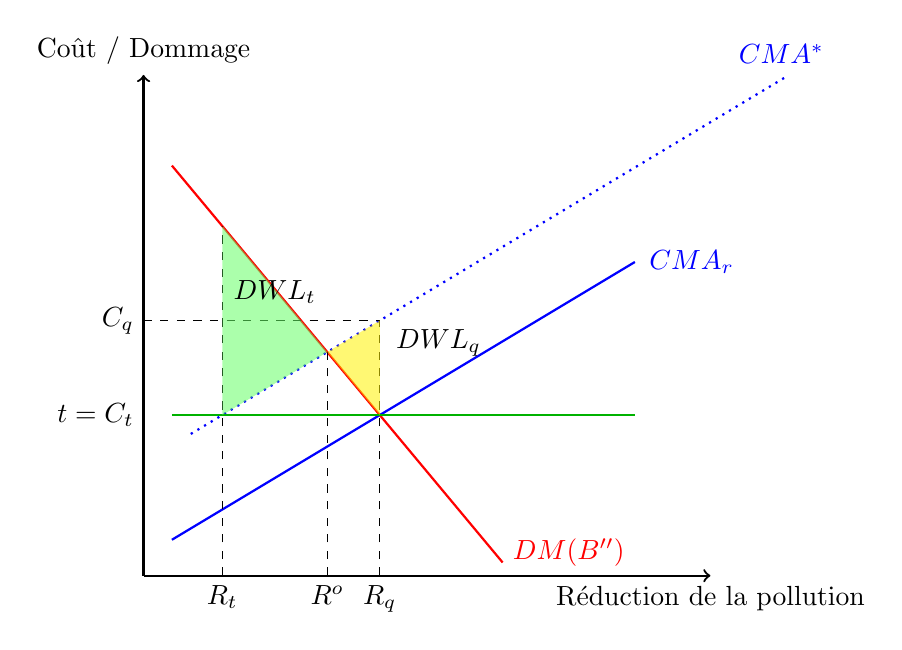
\begin{tikzpicture}[scale=1.2]
% Paramètres
\pgfmathsetmacro{\m}{0.6}        % pente des CMA
\pgfmathsetmacro{\bE}{0.2}       % intercept CMAr
\pgfmathsetmacro{\bA}{1.2}       % intercept CMA*

% Point de pivot fixe : intersection CMAr et taxe
% On choisit Rt = 2.5 comme point de pivot
\pgfmathsetmacro{\Rpivot}{2.5}
\pgfmathsetmacro{\tlevel}{\m*\Rpivot+\bE}  % taxe passe par CMAr au pivot

% Nouvelle pente pour DM (beaucoup plus pentu)
\pgfmathsetmacro{\d}{1.2}

% Recalculer k pour que MD passe par le point de pivot (Rpivot, tlevel)
\pgfmathsetmacro{\k}{\tlevel + \d*\Rpivot}

% Points clés
% R* (optimal) : intersection CMA* et MD
\pgfmathsetmacro{\Ro}{(\k-\bA)/(\m+\d)}
\pgfmathsetmacro{\yRo}{\m*\Ro+\bA}

% Rt : intersection CMA* et taxe (à gauche de R*)
\pgfmathsetmacro{\Rt}{(\tlevel-\bA)/\m}
\pgfmathsetmacro{\yMDatRt}{\k-\d*\Rt}

% Rq : intersection CMAr et MD (à droite de R*)
\pgfmathsetmacro{\Rq}{(\k-\bE)/(\m+\d)}
\pgfmathsetmacro{\yRq}{\m*\Rq+\bE}
\pgfmathsetmacro{\Cq}{\m*\Rq+\bA}  % coût sur CMA* à Rq

% Axes
\draw[->, thick] (0,0) -- (6,0) node[below] {Réduction de la pollution};
\draw[->, thick] (0,0) -- (0,5.3) node[above] {Coût / Dommage};

% Courbe CMA* (bleu pointillé)
\draw[thick, blue, dotted] (0.5, {\m*0.5+\bA}) -- (6.8, {\m*6.8+\bA});
\node[blue] at (6.75, {\m*7.2+\bA}) {$CMA^*$};

\draw[thick, blue] (0.3, {\m*0.3+\bE}) -- (5.2, {\m*5.2+\bE});
\node[blue] at (5.8, {\m*5.2+\bE}) {$CMA_r$};

% Courbe DM (pente négative forte)
\draw[thick, red] (0.3, {\k-\d*0.3}) -- (3.8, {\k-\d*3.8});
\node[red] at (4.5, {\k-\d*3.8+0.1}) {$DM (B'')$};

% Taxe (horizontale passant par le pivot)
\draw[thick, green!70!black] (0.3,\tlevel) -- (5.2,\tlevel);
\node[left] at (0,\tlevel) {$t=C_t$};

% Verticales
\draw[dashed] (\Rt,0) -- (\Rt,\yMDatRt);
\node[below] at (\Rt,0) {$R_t$};

\draw[dashed] (\Ro,0) -- (\Ro,\yRo);
\node[below] at (\Ro,0) {$R^{o}$};

\draw[dashed] (\Rq,0) -- (\Rq,\Cq);
\node[below] at (\Rq,0) {$R_q$};

% Horizontale Cq
\draw[dashed] (0,\Cq) -- (\Rq,\Cq);
\node[left] at (0,\Cq) {$C_q$};

% DWL taxe : triangle entre Rt, R* sur les courbes
\fill[green!60, opacity=0.55]
  (\Rt,\tlevel) -- (\Ro,\yRo) -- (\Rt,\yMDatRt) -- cycle;
\node at ({(\Rt+\Ro)/2}, {(\tlevel+\yMDatRt)/2.4 + 0.75}) {$DWL_t$};

% DWL quota : triangle entre R*, Rq
\fill[yellow, opacity=0.55]
  (\Ro,\yRo) -- (\Rq,\yRq) -- (\Rq,\Cq) -- cycle;
\node at ({(\Ro+\Rq)/2 + 0.9}, {\yRo+0.1}) {$DWL_q$};

\end{tikzpicture}
\end{frame}



%========================
% Slide: Contingency table MAC vs MD
%========================
\begin{frame}{Prix ou quantité ? Rôle de la courbure des courbes}

\centering
\renewcommand{\arraystretch}{1.8} % plus d'espace vertical
\begin{tabular}{>{\centering\arraybackslash}m{3cm}|>{\centering\arraybackslash}m{3.5cm}|>{\centering\arraybackslash}m{3.5cm}}
\toprule
 & \textbf{CMA plats} \newline \small{($C''$ faible)} & \textbf{CMA raides} \newline \small{($C''$ élevé)} \\
\midrule
\textbf{DM plats} \newline \small{($|B''|$ faible)} 
& \cellcolor{gray!20} Instruments équivalents 
& \cellcolor{green!25} \textbf{Prix préférables} \\
\midrule
\textbf{DM raides} \newline \small{($|B''|$ élevé)} 
& \cellcolor{yellow!35} \textbf{Quantités préférables} 
& \cellcolor{gray!20} Instruments équivalents \\
\bottomrule
\end{tabular}

\vspace{0.5cm}

\begin{itemize}
  \item DM raides : erreurs de pollution très coûteuses $\Rightarrow$ quantités.
  \item CMA raides : erreurs de coûts très coûteuses $\Rightarrow$ prix.
\end{itemize}

\end{frame}


\begin{frame}{Conclusion : Prix vs Quantité}

\textbf{Résultat clé (Weitzman 1974)}
\begin{itemize}
    \item Régulation par les \textbf{prix} ou les \textbf{quantités} en fonction de la relation  $CMA'$ vs $ DM'$
\end{itemize}

\vspace{0.4cm}
\textbf{Limitation liées aux hypothèses sous-jacentes}
\begin{enumerate}
    \item \textbf{Hétérogénéité des firmes} : Un quota sans marché de permis devient plus inefficace avec des CMA hétérogènes.
    
    \item \textbf{Non-linéarité des dommages} : L'hypothèse de linéarité est questionnable face aux points de basculement climatiques ('tipping points') et une potentielle irreversibilité $\Rightarrow$ favorise la régulation par quantités.

\end{enumerate}

\vspace{0.4cm}
\textbf{Conclusion :} Pas de jugement définitif sur la supériorité d'un instrument, mais un cadre utile pour comprendre les arbitrages.

\end{frame}



\section{Growth models}

% Slide 1: Output as function of labor
\begin{frame}[plain,label=growth1]
  \Large
  \[
    Y = L
  \]
  \vspace{1em}
  \begin{itemize}\Large
    \item $Y$: output (GDP)
    \item $L$: labor (population)
  \end{itemize}
\end{frame}

% Slide 2: Include capital
\begin{frame}[plain,label=growth2]
  \Large
  \[
    Y = K \times L
  \]
  \vspace{1em}
  \begin{itemize}\Large
    \item $Y$: output (GDP)
    \item $L$: labor (population)
    \item $K$: capital (machines)
  \end{itemize}
\end{frame}

% Slide 3: Include technology
\begin{frame}[plain,label=growth3]
  \Large
  \[
    Y = A \times K \times L
  \]
  \vspace{1em}
  \begin{itemize}\Large
    \item $Y$: output (GDP)
    \item $L$: labor (population)
    \item $K$: capital (machines)
    \item $A$: technology (exogenous)
  \end{itemize}
\end{frame}

% Slide 4: Production & Savings → Investment
\begin{frame}[plain,label=growth4]
  \Large

  % Equation (1)
  \[
    \tag{1}\;Y = A \times K \times L
  \]

  \vspace{1em}

  % Equation (2)
  \[
    \tag{2}\;s \times Y = I = \Delta K
  \]
  \vspace{0.5em}
  \begin{itemize}\Large
    \item $s$: savings rate (fraction of output saved)
    \item $sY$: saved (unconsumed) output
    \item $I$: investment
    \item $\Delta K$: change in capital stock (new investment)
  \end{itemize}
\end{frame}

% Slide: Endogenizing Technology (A)
\begin{frame}[plain,label=growth5]
  \Large
  \[
    \tag{1}\;Y = A(t)\,\;K^\alpha\,L^{1-\alpha}
  \]
  \vspace{0.75em}
  \[
    \tag{2}\;\dot A = \underbrace{\phi\,A^\lambda\,L_A}_{\text{R\&D production}}\quad\Longrightarrow\quad
    \text{A grows without bound.}
  \]
  \vspace{0.5em}
  \begin{itemize}\Large
    \item In Solow: \(A\) exogenous, fixed  
    \item {\bf Romer (1990)}: \(\dot A=\phi\,A\,L_A\) (non-rival spillovers) 
    \item {\bf Lucas (1988)}: human-capital externality, \(\dot H = \psi\,H\,u_H\) with \(u_H\) in R\&D 
    \item {\bf Aghion–Howitt (1992)}: creative destruction, \(\dot A = \mu\,\bigl(\tfrac{K_R}{\bar K}\bigr)^\eta A\) from innovation races  
    \item Knowledge accumulation → perpetual, scale‐sensitive growth
  \end{itemize}
\end{frame}

\section{NPV, discount rate, LCOE}

\begin{frame}[label=nb1]{Net Benefits (Undiscounted)}

\textbf{Approach 1: Sum of Benefits minus Sum of Costs}
\[
NB = \left(\sum_{t=0}^{N} B_t\right) - \left(\sum_{t=0}^{N} C_t\right)
\]

\textbf{Approach 2: Sum of Net Benefits per Period}
\[
NB = \sum_{t=0}^{N} (B_t - C_t)
\]

\vspace{0.5cm}

\textbf{Three-Period Example (t = 0 to t = 2):}

\textbf{Approach 1:}
\[
NB = (B_0 + B_1 + B_2) - (C_0 + C_1 + C_2)
\]

\textbf{Approach 2:}
\[
NB = (B_0 - C_0) + (B_1 - C_1) + (B_2 - C_2)
\]

\end{frame}

\begin{frame}[label=npv1]{Net Present Value (Discounted)}

\textbf{Approach 1: PV of Benefits minus PV of Costs}
\[
NPV = \left(\sum_{t=0}^{N} \frac{B_t}{(1+r)^t}\right) - \left(\sum_{t=0}^{N} \frac{C_t}{(1+r)^t}\right)
\]

\textbf{Approach 2: Sum of Discounted Net Benefits}
\[
NPV = \sum_{t=0}^{N} \frac{(B_t - C_t)}{(1+r)^t}
\]

\vspace{0.5cm}

\textbf{Three-Period Example (t = 0 to t = 2):}

\textbf{Approach 1:}
\[
NPV = \left(B_0 + \frac{B_1}{(1+r)} + \frac{B_2}{(1+r)^2}\right) - \left(C_0 + \frac{C_1}{(1+r)} + \frac{C_2}{(1+r)^2}\right)
\]

\textbf{Approach 2:}
\[
NPV = (B_0 - C_0) + \frac{(B_1 - C_1)}{(1+r)} + \frac{(B_2 - C_2)}{(1+r)^2}
\]

\end{frame}


\begin{frame}[label=discount1]{Discount Rates: Different Perspectives}

\textbf{The Discount Factor:}
\[
d_t = \frac{1}{(1+r)^t}
\]

\vspace{0.3cm}

\textbf{Three Cases:}

\begin{itemize}
    \item \textbf{$r \rightarrow 0$ (Environmentalist/Ethical Case):} Present and future benefits/costs are equally weighted. Intergenerational equity: future generations matter as much as current generation.
    
    \item \textbf{$r > 0$ (Economist Case):} Preference for the present, reflecting opportunity costs and time preference.
    \begin{itemize}
        \item Stern Review: $r \approx 1.4\%$ (low pure time preference)
        \item Nordhaus: $r \approx 4.5\%$ (market-based approach)
    \end{itemize}
    
    \item \textbf{$r < 0$ (Theoretical Case):} Future benefits and costs weighted higher than present. Not used in practice but conceptually relevant for growing environmental damages.
\end{itemize}

\end{frame}

\begin{frame}[label=discount2]{Discount Rates: Example}

\textbf{Project with net benefit of \$1,000,000 received in 30 years}

\textbf{NPV calculation:}
\[
NPV = \frac{1,000,000}{(1+r)^{30}}
\]

\vspace{0.3cm}

\begin{table}[]
\centering
\begin{tabular}{lcc}
\hline
\textbf{Perspective} & \textbf{Discount Rate} & \textbf{NPV (\$)} \\
\hline
Environmentalist & $r = 0\%$ & 1,000,000 \\
Stern (Climate) & $r = 1.4\%$ & 659,000 \\
EPA/Social & $r = 3\%$ & 412,000 \\
Nordhaus & $r = 4.5\%$ & 267,000 \\
Private/Market & $r = 7\%$ & 131,000 \\
High Private & $r = 10\%$ & 57,000 \\
\hline
\end{tabular}
\end{table}

\vspace{0.2cm}
\small{Choice of discount rate dramatically affects project valuation!}

\end{frame}

\begin{frame}[label=lcoe1]{Levelized Cost of Energy (LCOE) - Private Costs}

\textbf{Standard LCOE Formula (Private Costs Only):}
\[
LCOE = \frac{\sum_{t=0}^{N} \frac{I_t + M_t + F_t}{(1+r)^t}}{\sum_{t=0}^{N} \frac{E_t}{(1+r)^t}}
\]

\vspace{0.3cm}

\textbf{Components:}
\begin{itemize}
    \item $I_t$ = Capital investment costs in year $t$ (construction, equipment)
    \item $M_t$ = Operations \& maintenance costs in year $t$ (labor, repairs)
    \item $F_t$ = Fuel costs in year $t$ (coal, gas, uranium; \$0 for renewables)
    \item $E_t$ = Electricity generated in year $t$ (MWh)
    \item $r$ = Discount rate (cost of capital)
    \item $N$ = Project lifetime (typically 20-40 years)
\end{itemize}

\vspace{0.2cm}
\textbf{Units:} Typically expressed in \$/MWh or \$/kWh

\end{frame}

\begin{frame}[label=lcoe2]{LCOE with External Costs}

\textbf{Social LCOE Formula (Including Carbon Price):}
\[
LCOE_{social} = \frac{\sum_{t=0}^{N} \frac{I_t + M_t + F_t + (CO2_t \times P_{carbon,t})}{(1+r)^t}}{\sum_{t=0}^{N} \frac{E_t}{(1+r)^t}}
\]

\vspace{0.3cm}

\textbf{Additional Components:}
\begin{itemize}
    \item $CO2_t$ = CO$_2$ emissions in year $t$ (tons)
    \item $P_{carbon,t}$ = Carbon price in year $t$ (\$/ton CO$_2$)
    \item Captures climate externality costs
\end{itemize}

\vspace{0.2cm}
\textbf{Note:} For comprehensive social LCOE, would also add health damages (PM$_{2.5}$, NO$_x$, SO$_2$), water use, land degradation, etc.

\end{frame}

\begin{frame}[label=lcoe3]{LCOE Example: Three-Period Case}

\textbf{Assumptions:} Coal plant, $r = 7\%$, 3 years (simplified)

\textbf{Without External Costs:}
\[
LCOE_{private} = \frac{1000 + \frac{50+30+40}{1.07} + \frac{50+30+40}{1.07^2}}{1000 + \frac{1000}{1.07} + \frac{1000}{1.07^2}}
\]
\[
= \frac{1000 + 112.1 + 104.8}{1000 + 934.6 + 873.4} = \frac{1216.9}{2808.0} = \$0.43/\text{MWh-unit}
\]

\vspace{0.3cm}

\textbf{With External Costs (Carbon Price = \$50/ton, 1 ton CO$_2$/MWh):}
\[
LCOE_{social} = \frac{1000 + \frac{50+30+40+50}{1.07} + \frac{50+30+40+50}{1.07^2}}{1000 + \frac{1000}{1.07} + \frac{1000}{1.07^2}}
\]
\[
= \frac{1000 + 158.9 + 148.5}{2808.0} = \frac{1307.4}{2808.0} = \$0.47/\text{MWh-unit}
\]

\small{External costs increase LCOE by $\sim$9\% in this example}

\end{frame}

\begin{frame}[label=lcoe4]{LCOE Example: Detailed Breakdown}

\textbf{Three-Period Example Details:}

\vspace{0.3cm}

\begin{table}[]
\centering
\small
\begin{tabular}{lcccc}
\hline
\textbf{Period} & \textbf{$I_t$} & \textbf{$M_t$} & \textbf{$F_t$} & \textbf{$E_t$} \\
\hline
$t=0$ & 1000 & 0 & 0 & 1000 MWh \\
$t=1$ & 0 & 50 & 30+40=70 & 1000 MWh \\
$t=2$ & 0 & 50 & 30+40=70 & 1000 MWh \\
\hline
\end{tabular}
\end{table}

\vspace{0.3cm}

\textbf{Carbon Externality:}
\begin{itemize}
    \item Coal emissions: 1 ton CO$_2$ per MWh
    \item Carbon price: \$50/ton
    \item Annual external cost: 1000 MWh $\times$ 1 ton/MWh $\times$ \$50/ton = \$50
\end{itemize}

\vspace{0.2cm}

\textbf{Key Insight:} Renewable energy (solar/wind) has $F_t = 0$ and $CO2_t = 0$, making social LCOE $\approx$ private LCOE

\end{frame}

\begin{frame}[label=altdisc1]{Alternative Discount Rate Approaches for Environmental Costs}

\textbf{The Problem:} Standard discounting may undervalue environmental damages because:
\begin{itemize}
    \item Irreversible damages (extinction, ecosystem collapse)
    \item Intergenerational equity concerns
    \item Growing marginal damages over time
    \item Non-substitutability of natural capital
\end{itemize}

\vspace{0.3cm}

\textbf{Three Alternative Approaches:}
\begin{enumerate}
    \item Dual/Differential Discounting
    \item Declining Discount Rates
    \item Shadow Price with Growing Damages
\end{enumerate}

\end{frame}

\begin{frame}[label=dual1]{Option 1: Dual/Differential Discounting}

\textbf{Concept:} Use different discount rates for different types of impacts

\[
NPV = \sum_{t=0}^{N} \frac{B_t}{(1+r_{financial})^t} - \sum_{t=0}^{N} \frac{C_t}{(1+r_{financial})^t} - \sum_{t=0}^{N} \frac{D_t^{env}}{(1+r_{environmental})^t}
\]

Where: $r_{financial} > r_{environmental}$

\vspace{0.3cm}

\textbf{Typical Values:}
\begin{itemize}
    \item Financial costs/benefits: $r = 3-7\%$
    \item Environmental damages: $r = 0-2\%$
\end{itemize}

\vspace{0.3cm}

\textbf{Rationale:} Environmental goods become relatively scarcer over time; low substitutability with market goods; ethical obligations to future generations

\end{frame}

\begin{frame}[label=dual2]{Dual Discounting: Key References}

\textbf{Foundational Papers:}

\begin{itemize}
    \small
    \item \textbf{Weitzman, M.L. (1994).} "On the 'Environmental' Discount Rate." \textit{Journal of Environmental Economics and Management}, 26(2), 200-209.
    
    \item \textbf{Gollier, C. (2010).} "Ecological discounting." \textit{Journal of Economic Theory}, 145(2), 812-829.
    
    \item \textbf{Hoel, M. \& Sterner, T. (2007).} "Discounting and relative prices." \textit{Climatic Change}, 84(3-4), 265-280.
    
    \item \textbf{Traeger, C.P. (2011).} "Sustainability, limited substitutability, and non-constant social discount rates." \textit{Journal of Environmental Economics and Management}, 62(2), 215-228.
    
    \item \textbf{Weikard, H.P. \& Zhu, X. (2005).} "Discounting and environmental quality: When should dual rates be used?" \textit{Economic Modelling}, 22(5), 868-878.
    
    \item \textbf{Baumgärtner, S. et al. (2015).} "Trade-offs between justices and efficiency." \textit{Environmental and Resource Economics}, 60, 97-118.
\end{itemize}

\end{frame}

\begin{frame}[label=ddr1]{Option 2: Declining Discount Rates (DDR)}

\textbf{Concept:} Discount rate decreases over time horizon

\[
NPV = \sum_{t=0}^{N} \frac{(B_t - C_t)}{(1+r_t)^t}
\]

Where: $r_t = r_0 \cdot e^{-\gamma t}$ or use step function

\vspace{0.3cm}

\textbf{Example (UK Green Book):}
\begin{table}[]
\small
\begin{tabular}{ll}
\hline
\textbf{Time Period} & \textbf{Discount Rate} \\
\hline
Years 0-30 & 3.5\% \\
Years 31-75 & 3.0\% \\
Years 76-125 & 2.5\% \\
Years 126-200 & 2.0\% \\
Years 201-300 & 1.5\% \\
Years 301+ & 1.0\% \\
\hline
\end{tabular}
\end{table}

\vspace{0.2cm}

\textbf{Rationale:} Uncertainty about future discount rates; precautionary principle; intergenerational equity

\end{frame}

\begin{frame}[label=ddr2]{Declining Discount Rates: Key References}

\textbf{Foundational Papers:}

\begin{itemize}
    \small
    \item \textbf{Weitzman, M.L. (1998).} "Why the far-distant future should be discounted at its lowest possible rate." \textit{Journal of Environmental Economics and Management}, 36(3), 201-208.
    
    \item \textbf{Weitzman, M.L. (2001).} "Gamma discounting." \textit{American Economic Review}, 91(1), 260-271.
    
    \item \textbf{Gollier, C. (2002).} "Time horizon and the discount rate." \textit{Journal of Economic Theory}, 107(2), 463-473.
    
    \item \textbf{Newell, R.G. \& Pizer, W.A. (2003).} "Discounting the distant future: how much do uncertain rates increase valuations?" \textit{Journal of Environmental Economics and Management}, 46(1), 52-71.
    
    \item \textbf{Arrow, K.J. et al. (2013).} "Determining benefits and costs for future generations." \textit{Science}, 341(6144), 349-350.
    
    \item \textbf{Groom, B. et al. (2005).} "Declining discount rates: the long and the short of it." \textit{Environmental and Resource Economics}, 32(4), 445-493.
\end{itemize}

\end{frame}

\begin{frame}[label=shadow1]{Option 3: Shadow Price with Growing Marginal Damages}

\textbf{Concept:} Don't discount damages directly; discount shadow price of carbon which accounts for growing damages

\[
SCC_t = \sum_{s=t}^{N} \frac{MD_s(Stock_s)}{(1+r)^{s-t}}
\]

Where:
\begin{itemize}
    \item $MD_s$ = Marginal damage at time $s$ (depends on cumulative stock)
    \item $Stock_s$ = $Stock_{s-1} + Emissions_s - Decay_s$
    \item Damages grow non-linearly as stock accumulates
\end{itemize}

\vspace{0.3cm}

\textbf{Key insight:} Even with positive $r$, if $MD_s$ grows faster than discount rate, present value of future damages increases

\textbf{Example:} US Government Social Cost of Carbon
\begin{itemize}
    \item 2020: \$51/ton CO$_2$ → 2050: \$85/ton (real terms, at 3\% discount)
\end{itemize}

\end{frame}

\begin{frame}[label=shadow2]{Shadow Price Approach: Key References}

\textbf{Foundational Papers:}

\begin{itemize}
    \small
    \item \textbf{Interagency Working Group (2021).} "Technical Support Document: Social Cost of Carbon, Methane, and Nitrous Oxide." US Government.
    
    \item \textbf{Dietz, S. \& Stern, N. (2015).} "Endogenous growth, convexity of damage and climate risk: How Nordhaus' framework supports deep cuts in carbon emissions." \textit{Economic Journal}, 125(583), 574-620.
    
    \item \textbf{Pindyck, R.S. (2013).} "Climate change policy: What do the models tell us?" \textit{Journal of Economic Literature}, 51(3), 860-872.
    
    \item \textbf{National Academies (2017).} \textit{Valuing Climate Damages: Updating Estimation of the Social Cost of Carbon Dioxide.} Washington, DC: National Academies Press.
    
    \item \textbf{Rennert, K. et al. (2022).} "Comprehensive evidence implies a higher social cost of CO$_2$." \textit{Nature}, 610, 687-692.
\end{itemize}

\vspace{0.2cm}

\textbf{Policy Documents:}
\begin{itemize}
    \small
    \item UK HM Treasury Green Book (2022)
    \item World Bank Shadow Price of Carbon Guidance (2024)
\end{itemize}

\end{frame}

\begin{frame}[label=comparison]{Comparison of Three Approaches}

\begin{table}[]
\tiny
\begin{tabular}{p{2cm}p{3cm}p{3cm}p{3cm}}
\hline
\textbf{Approach} & \textbf{Mechanism} & \textbf{Advantages} & \textbf{Challenges} \\
\hline
\textbf{Dual Rates} & Different $r$ for environmental vs. financial & Simple; reflects scarcity; ethical foundation & Theoretically contentious; arbitrary rate selection \\
\hline
\textbf{Declining Rates} & $r_t$ decreases over time & Captures uncertainty; UK/France adopted & Time inconsistency issues; complex implementation \\
\hline
\textbf{Shadow Price} & Damages grow in numerator & Theoretically consistent; used by US govt & Requires damage function modeling; high uncertainty \\
\hline
\end{tabular}
\end{table}

\vspace{0.3cm}

\textbf{Common Thread:} All three approaches give greater weight to distant future environmental damages than standard constant discounting at market rates (3-7\%)

\vspace{0.2cm}

\textbf{Policy Adoption:}
\begin{itemize}
    \item UK: Declining rates (Green Book)
    \item US: Shadow price approach (SCC)
    \item France: Combination of approaches
    \item World Bank: Shadow price guidance for client countries
\end{itemize}

\end{frame}

\section{Cap and Trade System: Part A}

\begin{frame}{Setting up the System of Equations}

We have two equations with two unknowns ($Q_A$ and $Q_B$):

\vspace{0.5cm}

\textbf{Equation 1 (Total abatement constraint):}
\begin{equation}
Q_A + Q_B = 50
\end{equation}

\vspace{0.5cm}

\textbf{Equation 2 (Equal MAC condition):}
\begin{equation}
2Q_A + 0.5Q_A^2 = Q_B + 0.2Q_B^2
\end{equation}
\end{frame}

\begin{frame}{Solving the System: Steps 1-2}

\textbf{Step 1: Express $Q_A$ in terms of $Q_B$}

From Equation 1:
\begin{equation}
Q_A = 50 - Q_B
\end{equation}

\vspace{0.5cm}

\textbf{Step 2: Substitute into Equation 2}

\begin{equation}
2(50 - Q_B) + 0.5(50 - Q_B)^2 = Q_B + 0.2Q_B^2
\end{equation}

\end{frame}

\begin{frame}{Mathematical Tools and Expansion}
\textbf{Algebraic Identities:}
\begin{align}
(a + b)^2 &= a^2 + 2ab + b^2 \\
(a - b)^2 &= a^2 - 2ab + b^2
\end{align}
\vspace{0.3cm}
\textbf{Quadratic Formula:}
\begin{equation}
\text{For } ax^2 + bx + c = 0, \quad x = \frac{-b \pm \sqrt{b^2 - 4ac}}{2a}
\end{equation}
\end{frame}


\begin{frame}{Mathematical Tools and Expansion}

\textbf{Algebraic Identities:}
\begin{align}
(a + b)^2 &= a^2 + 2ab + b^2 \\
(a - b)^2 &= a^2 - 2ab + b^2
\end{align}

\textit{Example from our problem:}
$$(50 - Q_B)^2 = 50^2 - 2(50)(Q_B) + Q_B^2 = 2500 - 100Q_B + Q_B^2$$

\vspace{0.3cm}

\textbf{Quadratic Formula:}
\begin{equation}
\text{For } ax^2 + bx + c = 0, \quad x = \frac{-b \pm \sqrt{b^2 - 4ac}}{2a}
\end{equation}

\textit{Example from our problem:}
$$0.3Q_B^2 - 53Q_B + 1350 = 0$$
$$\text{where } a = 0.3, \; b = -53, \; c = 1350$$

\end{frame}

\begin{frame}{Step 3: Expand the Binomial Term}

\textbf{Starting equation:}
$$2(50 - Q_B) + \colorbox{red!30}{$0.5(50 - Q_B)^2$} = Q_B + 0.2Q_B^2$$

\vspace{0.2cm}

\textbf{Algebraic Identities:}
\begin{align}
(a + b)^2 &= a^2 + 2ab + b^2 \\
(a - b)^2 &= a^2 - 2ab + b^2
\end{align}

\vspace{0.2cm}

\textbf{Solve the identity term } $\colorbox{red!30}{$(50 - Q_B)^2$}$:
\begin{align}
(50 - Q_B)^2 &= 50^2 - 2(50)(Q_B) + Q_B^2 \\
&= 2500 - 100Q_B + Q_B^2
\end{align}

Therefore:
\begin{align}
0.5(50 - Q_B)^2 &= 0.5(2500 - 100Q_B + Q_B^2) \\
&= 1250 - 50Q_B + 0.5Q_B^2
\end{align}

\end{frame}

\begin{frame}{Step 4: Substitute and Rearrange}

\textbf{Original equation:}
$$2(50 - Q_B) + \colorbox{red!30}{$0.5(50 - Q_B)^2$} = Q_B + 0.2Q_B^2$$

\vspace{0.3cm}

\textbf{Substitute the expanded term:}
$$100 - 2Q_B + \colorbox{red!30}{$1250 - 50Q_B + 0.5Q_B^2$} = Q_B + 0.2Q_B^2$$

\vspace{0.3cm}

\textbf{Rearrange to standard quadratic form } $ax^2 + bx + c = 0$:
$$0.3Q_B^2 - 53Q_B + 1350 = 0$$

\end{frame}


\begin{frame}{Step 5: Using Quadratic Formula to Calculate $Q_B^*$}

\textbf{Quadratic equation:}
$$0.3Q_B^2 - 53Q_B + 1350 = 0$$

where $a = 0.3$, $b = -53$, $c = 1350$

\vspace{0.3cm}

\textbf{Apply quadratic formula:}
$$Q_B = \frac{-b \pm \sqrt{b^2 - 4ac}}{2a} = \frac{-(-53) \pm \sqrt{(-53)^2 - 4(0.3)(1350)}}{2(0.3)}$$

$$Q_B = \frac{53 \pm \sqrt{2809 - 1620}}{0.6} = \frac{53 \pm \sqrt{1189}}{0.6}$$

$$Q_B = \frac{53 \pm 34.48}{0.6}$$

\textbf{Two solutions:}
$$Q_B = \frac{53 + 34.48}{0.6} = 145.8 \quad \text{or} \quad Q_B^* = \frac{53 - 34.48}{0.6} = 30.87 \text{ tons}$$

\end{frame}




\begin{frame}{Step 6: Using Optimal $Q_B^*$ to Get $Q_A^*$}

\textbf{From the constraint equation:}
$$Q_A + Q_B = 50$$

\vspace{0.3cm}

\textbf{Substitute } $Q_B^* = 30.87$ tons:
$$Q_A^* = 50 - Q_B^*$$

$$Q_A^* = 50 - 30.87$$

$$Q_A^* = 19.13 \text{ tons}$$

\end{frame}

\begin{frame}{Step 7: Using MAC to Calculate $P^*$}

\textbf{Using Plant B's MAC equation:}
$$P^* = Q_B + 0.2Q_B^2 = 30.87 + 0.2(30.87)^2$$

$$P^* = 30.87 + 0.2(952.96) = 30.87 + 190.59$$

$$P^* = \$221.46 \text{ per ton}$$

\vspace{0.5cm}

\textbf{Verification using Plant A's MAC equation:}
$$P^* = 2Q_A + 0.5Q_A^2 = 2(19.13) + 0.5(19.13)^2$$

$$P^* = 38.26 + 0.5(365.96) = 38.26 + 182.98$$

$$P^* = \$221.24 \text{ per ton} \quad \checkmark$$

\end{frame}


\begin{frame}{Step 8: Permits and Emission Levels}

\textbf{Initial permit allocation (50 tons each):}
\begin{itemize}
    \item Plant A (Coal): 50 tons
    \item Plant B (Gas): 50 tons
    \item Total: 100 tons
\end{itemize}

\vspace{0.3cm}

\textbf{Actual emissions after abatement:}
\begin{align}
\text{Plant A (Coal) emissions} &= \text{Baseline} - Q_A^* = 100 - 19.13 = 80.87 \text{ tons} \\
\text{Plant B (Gas) emissions} &= \text{Baseline} - Q_B^* = 50 - 30.87 = 19.13 \text{ tons}
\end{align}

\vspace{0.3cm}

\textbf{Permit trading:}
\begin{itemize}
    \item Plant A (Coal) needs: $80.87 - 50 = 30.87$ permits (buyer)
    \item Plant B (Gas) has surplus: $50 - 19.13 = 30.87$ permits (seller)
\end{itemize}

\end{frame}

\begin{frame}{Step 9: Abatement and Permit Costs Calculation}

\textbf{Abatement Costs (TAC) = } $\int_0^{Q^*} MAC \, dQ$

\textbf{Plant A (Coal):}
$$TAC_A = \int_0^{19.13} (2Q + 0.5Q^2) dQ = \left[Q^2 + \frac{Q^3}{6}\right]_0^{19.13} = \$1,533.40$$

\textbf{Plant B (Gas):}
$$TAC_B = \int_0^{30.87} (Q + 0.2Q^2) dQ = \left[\frac{Q^2}{2} + \frac{Q^3}{15}\right]_0^{30.87} = \$2,437.80$$

\vspace{0.3cm}

\textbf{Permit Costs/Revenue at } $P^* = \$221.46$ per ton:

\textbf{Plant A (Coal):} Buys 30.87 permits
$$\text{Permit Cost}_A = 30.87 \times 221.46 = \$6,836.47$$

\textbf{Plant B (Gas):} Sells 30.87 permits
$$\text{Permit Revenue}_B = 30.87 \times 221.46 = \$6,836.47$$

\end{frame}

\begin{frame}{Step 10: Cost Comparison Summary}

\begin{table}
\begin{tabular}{lccc}
\hline
\textbf{Component} & \textbf{Plant A (Coal)} & \textbf{Plant B (Gas)} \\
\hline
Abatement (tons) & 19.13 & 30.87 \\[0.2cm]
Abatement Cost & \$1,533.40 & \$2,437.80 \\[0.2cm]
Permit Cost/Revenue & -\$6,836.47 & +\$6,836.47 \\
 & (buys 30.87) & (sells 30.87) \\[0.2cm]
\hline
\textbf{Net Position} & \textbf{\textcolor{red}{-\$8,369.87}} & \textbf{\textcolor{green!50!black}{+\$4,398.67}} \\
\hline
\end{tabular}
\end{table}

\vspace{0.5cm}

\textbf{Key Insights:}
\begin{itemize}
    \item Plant B abates more (lower MAC) and earns net revenue
    \item Plant A abates less but incurs higher total costs
    \item Cap-and-trade achieves cost-effective 50-ton reduction
    \item Permit market transfers \$6,836.47 from Plant A to Plant B
\end{itemize}

\end{frame}



\section{Cap and Trade System: Part B}

\begin{frame}{Question 2: System of Equations for Equilibrium}

\textbf{Answer:}

The equilibrium is characterized by two equations:

\vspace{0.3cm}

\textbf{Equation 1 (Equilibrium condition):}
$$MAC_M = MAC_O = P^*$$

Which gives us:
$$2Q_M = 4Q_O = P^*$$

\vspace{0.3cm}

\textbf{Equation 2 (Total abatement constraint):}
$$Q_M + Q_O = 50$$

\end{frame}



\begin{frame}{Question 3: Equilibrium Permit Price}

\textbf{Answer:}

From the equilibrium conditions:
\begin{align}
MAC_M = P^* \quad &\Rightarrow \quad 2Q_M = P^* \quad \Rightarrow \quad Q_M = \frac{P^*}{2} \\
MAC_O = P^* \quad &\Rightarrow \quad 4Q_O = P^* \quad \Rightarrow \quad Q_O = \frac{P^*}{4}
\end{align}

Substitute into the total abatement constraint:
$$Q_M + Q_O = 50$$
$$\frac{P^*}{2} + \frac{P^*}{4} = 50$$

Solve for P*:
$$\frac{3P^*}{4} = 50 \quad \Rightarrow \quad P^* = \frac{50 \times 4}{3} = \$66.67 \text{ per ton}$$

\end{frame}



\begin{frame}{Question 4: Abatement by Each Plant}

\textbf{Answer:}

Using $P^* = \$66.67$:

\vspace{0.3cm}

\textbf{Modern Cement:}
$$Q_M = \frac{P^*}{2} = \frac{66.67}{2} = 33.33 \text{ tons}$$

\vspace{0.3cm}

\textbf{Old Cement:}
$$Q_O = \frac{P^*}{4} = \frac{66.67}{4} = 16.67 \text{ tons}$$

\vspace{0.3cm}

\textbf{Verification:} $33.33 + 16.67 = 50$ tons $\checkmark$

\end{frame}


\begin{frame}{Question 5: Emissions, Permit Needs, and Trading}

\textbf{Answer:}

\textbf{Modern Cement:}
\begin{itemize}
    \item Emissions = $100 - 33.33 = 66.67$ tons
    \item Permits needed: 66.67 permits
    \item Has: 50 permits (initial allocation)
    \item Action: \textbf{Buys 16.67 permits}
\end{itemize}

\vspace{0.3cm}

\textbf{Old Cement:}
\begin{itemize}
    \item Emissions = $50 - 16.67 = 33.33$ tons
    \item Permits needed: 33.33 permits
    \item Has: 50 permits (initial allocation)
    \item Action: \textbf{Sells 16.67 permits}
\end{itemize}

\end{frame}

\begin{frame}{Question 6: Total Abatement Costs, Trading, and Net Position}

\textbf{Answer:}

\textbf{Total Abatement Costs:} $TAC = \int_0^{Q^*} MAC \, dQ$

\textbf{Modern Cement:}
$$TAC_M = \int_0^{33.33} 2Q \, dQ = \left[Q^2\right]_0^{33.33} = (33.33)^2 = \$1,111.11$$

\textbf{Old Cement:}
$$TAC_O = \int_0^{16.67} 4Q \, dQ = \left[2Q^2\right]_0^{16.67} = 2(16.67)^2 = \$555.56$$

\vspace{0.3cm}

\textbf{Permit Trading at } $P^* = \$66.67$ per ton:
\begin{itemize}
    \item Modern Cement (Buyer): $16.67 \times 66.67 = \$1,111.11$ (cost)
    \item Old Cement (Seller): $16.67 \times 66.67 = \$1,111.11$ (revenue)
\end{itemize}

\vspace{0.3cm}

\textbf{Net Cost Position:}
\begin{itemize}
    \item Modern Cement: $\$1,111.11 + \$1,111.11 = \$2,222.22$
    \item Old Cement: $\$555.56 - \$1,111.11 = -\$555.56$ (net revenue)
\end{itemize}

\end{frame}





\section{Marginal user costs}

\begin{frame}{Demand and Marginal Cost}
\begin{center}
\begin{tikzpicture}
    \begin{axis}[
        width=8cm,
        height=8cm,
        xlabel={Quantity\\(units)},
        ylabel={Price\\(dollars\\per unit)},
        xmin=0, xmax=22,
        ymin=0, ymax=9,
        xtick={0,5,10,15,20},
        ytick={0,2,4,6,8},
        axis lines=left,
        xlabel style={align=center},
        ylabel style={align=center},
        every axis plot/.append style={thick},
        clip=false
    ]
    
    % Demand curve (from (0,8) to (20,0))
    \addplot[black, domain=0:20, samples=2] {8 - 0.4*x};
    \node[right] at (axis cs:1,8) {$MB$};

    % Marginal Cost line (horizontal at y=2)
    \addplot[black, domain=0:20, samples=2] {2};
    \node[right] at (axis cs:20,2) {$MC$};
    
    % Vertical dotted line at x=15
    %\draw[dotted, thick] (axis cs:15,0) -- (axis cs:15,2);
    
    % Label for part (a)
    %\node[below] at (axis cs:10,-1) {(a)};
    
    \end{axis}
\end{tikzpicture}
\end{center}
\end{frame}

%% EXERCISE 1 SLIDE
\begin{frame}{Exercise 1: Static Efficiency Problem}
\textbf{Question:} Calculate $q^*$ as the intersection of demand-supply (MB(q) = MC(q)) as if this were a static problem (not taking into account resource stock and two periods)?

\vspace{0.3cm}
\textbf{Solution:}
\begin{align*}
MB(q) &= MC(q)\\
8 - 0.4q &= 2\\
0.4q &= 6\\
q^* &= 15 \text{ units}
\end{align*}

\vspace{0.3cm}
\textbf{Remaining stock for period 2:}
$$20 - 15 = 5 \text{ units}$$

\vspace{0.3cm}
\alert{Are 5 units sufficient to cover the same consumption as in period 1?}

\textbf{No!} We would need 15 units in period 2, but only 5 units remain. This demonstrates the \textbf{myopic nature} of static efficiency when dealing with finite resources.
\end{frame}

%% EXERCISE 2A SLIDE
\begin{frame}{Exercise 2A: Setting Up the Dynamic Problem}
\textbf{Question:} Insert all elements from the set-up in equation 1) and write up the equation.

% \vspace{0.3cm}
% \textbf{Given:}
% \begin{itemize}
%     \item Equation 1: $PV(MB_1 - MC_1) = PV(MB_2 - MC_2)$
%     \item Demand: $P = 8 - 0.4q$
%     \item Marginal Cost: $MC = 2$
%     \item Discount rate: $r = 0.1$
% \end{itemize}

\vspace{0.3cm}
\textbf{Solution:}

\textbf{Left side (Period 1):}
$$PV(MB_1 - MC_1) = (8 - 0.4q_1) - 2 = 6 - 0.4q_1$$

\textbf{Right side (Period 2):}
$$PV(MB_2 - MC_2) = \frac{(8 - 0.4q_2) - 2}{1 + 0.1} = \frac{6 - 0.4q_2}{1.1}$$

\vspace{0.3cm}
\textbf{Complete equation:}
$$\boxed{6 - 0.4q_1 = \frac{6 - 0.4q_2}{1.1}}$$
\end{frame}

%% EXERCISE 2B SLIDE
\begin{frame}{Exercise 2B: Incorporating the Stock Constraint}
\textbf{Question:} Replace $q_2$ with its expression in terms of $q_1$ from equation 2.

\vspace{0.3cm}
\textbf{Given:}
\begin{itemize}
    \item Stock constraint: $20 = q_1 + q_2$
    \item Therefore: $q_2 = 20 - q_1$
\end{itemize}

\vspace{0.3cm}
\textbf{Solution:}

Starting from:
$$6 - 0.4q_1 = \frac{6 - 0.4q_2}{1.1}$$

Substitute $q_2 = 20 - q_1$:
$$\boxed{6 - 0.4q_1 = \frac{6 - 0.4(20 - q_1)}{1.1}}$$

Simplifying the right side:
$$\boxed{6 - 0.4q_1 = \frac{6 - 8 + 0.4q_1}{1.1} = \frac{-2 + 0.4q_1}{1.1}}$$
\end{frame}

%% EXERCISE 2C SLIDE
\begin{frame}{Exercise 2C: Solving for $q_1^*$}
\textbf{Question:} Solve for $q_1$.

\vspace{0.3cm}
\textbf{Solution:}

Starting from:
$$6 - 0.4q_1 = \frac{-2 + 0.4q_1}{1.1}$$

Multiply both sides by 1.1:
$$1.1(6 - 0.4q_1) = -2 + 0.4q_1$$
$$6.6 - 0.44q_1 = -2 + 0.4q_1$$

Collect terms with $q_1$:
$$6.6 + 2 = 0.4q_1 + 0.44q_1$$
$$8.6 = 0.84q_1$$

Solve for $q_1$:
$$\boxed{q_1^* = \frac{8.6}{0.84} \approx 10.24 \text{ units}}$$
\end{frame}

%% EXERCISE 2D SLIDE
\begin{frame}{Exercise 2D: Solving for $q_2^*$}
\textbf{Question:} Replace $q_1^*$ in equation 2 to get the optimal quantity extracted in period 2.

\vspace{0.3cm}
\textbf{Solution:}

Using the stock constraint:
$$q_2 = 20 - q_1$$

Substitute $q_1^* = 10.24$:
$$q_2^* = 20 - 10.24$$
$$\boxed{q_2^* = 9.76 \text{ units}}$$

\vspace{0.5cm}
\textbf{Key Insights:}
\begin{itemize}
    \item We extract \textbf{slightly more} in period 1 (10.24) than period 2 (9.76)
    \item This reflects the \textbf{time value of money} (discount rate = 10\%)
    \item Total extraction: $10.24 + 9.76 = 20$ units ✓
    \item Compare to static solution: 15 + 15 = 30 units (infeasible!)
\end{itemize}
\end{frame}



\end{document}